\documentclass[aspectratio=169]{beamer}
\newif\ifdraft
\draftfalse
\usepackage{style}
\addbibresource{references.bib}
\title[Title]{Extremal independent Set Reconfiguration}
\subtitle{ Nicolas Bousquet, Bastien Durain, Théo Pierron, Stéphan Thomassé}

% \subtitle{Subtitle}

\author{Andrzej Antoni Kwaśniewski \\ 
Advisor: Clément Legrand – Duchesne}
\date[]{Combinatorics 23 I 2026}
\begin{document}
\onehalfspacing
%---------------------------------------------------------

\frame{\titlepage}

%---------------------------------------------------------
\section{Preliminaries}
\begin{frame}{Reconfiguration problems}
    \begin{heading}{What are they?}
Ask whether one configuration can be transformed into another via a sequence of local, legal moves.
    \end{heading}
    \begin{heading}{Examples of reconfiguration problems}
    \begin{itemize}
        \item Rubik's cube
        \item Sokoban
        \item Graph recolouring reconfiguration
        \item Independent set reconfiguration
    \end{itemize}
    \end{heading}
    \pause
    Most reconfiguration problems don't belong in NP
\end{frame}

%--------------------------------------------

\begin{frame}{Independent set reconfiguration}
        Given two independent sets of size \(k\), is it possible to transform one into the other by changing vertices one by one in such a way that intermediate sets remain independent?
    \vspace{1em}
    \pause
    \begin{heading}{Two paradigms}
    \begin{itemize}
        \item Token sliding - only allows swaps within edges
        \item Token jumping - allows any swaps preserving independence
    \end{itemize}
    \end{heading}

    Both are PSPACE-complete
\end{frame}

%--------------------------------------------

\begin{frame}{Example: Token jumping reconfiguration}
\begin{figure}
\centering
\begin{tikzpicture}[scale=2]

% coordinates (defined once)
\coordinate (c1) at (1,2);
\coordinate (c2) at (3,2);
\coordinate (c3) at (0,1);
\coordinate (c4) at (2,1);
\coordinate (c5) at (4,1);
\coordinate (c6) at (1,0);
\coordinate (c7) at (3,0);

% edges (drawn once)
\draw[line width=1.5pt, dashed] (c1)--(c2);
\draw[line width=1.5pt, dashed] (c1)--(c3);
\draw[line width=1.5pt, dashed] (c1)--(c4);
\draw[line width=1.5pt, dashed] (c3)--(c6);
\draw[line width=1.5pt, dashed] (c1)--(c6);
\draw[line width=1.5pt, dashed] (c4)--(c6);
\draw[line width=1.5pt, dashed] (c2)--(c4);
\draw[line width=1.5pt, dashed] (c2)--(c5);
\draw[line width=1.5pt, dashed] (c2)--(c7);
\draw[line width=1.5pt, dashed] (c4)--(c7);
\draw[line width=1.5pt, dashed] (c5)--(c7);
\draw[line width=1.5pt, dashed] (c6)--(c7);

\only<1>{
    \node[circle,draw,fill=cfgr,minimum size=0.6cm,line width=1.5pt] at (c1) {};
    \node[circle,draw,fill=cfblue,minimum size=0.6cm,line width=1.5pt] at (c2) {};
    \node[circle,draw,fill=cfgr,minimum size=0.6cm,line width=1.5pt] at (c3) {};
    \node[circle,draw,fill=white,minimum size=0.6cm,line width=1.5pt] at (c4) {};
    \node[circle,draw,fill=cfblue,minimum size=0.6cm,line width=1.5pt] at (c5) {};
    \node[circle,draw,fill=cfgr,minimum size=0.6cm,line width=1.5pt] at (c6) {};
    \node[circle,draw,fill=cfblue,minimum size=0.6cm,line width=1.5pt] at (c7) {};
}

\only<2>{
    \node[circle,draw,fill=cfred,minimum size=0.6cm,line width=1.5pt] at (c1) {};
    \node[circle,draw,fill=white,minimum size=0.6cm,line width=1.5pt] at (c2) {};
    \node[circle,draw,fill=cfred,minimum size=0.6cm,line width=1.5pt] at (c3) {};
    \node[circle,draw,fill=white,minimum size=0.6cm,line width=1.5pt] at (c4) {};
    \node[circle,draw,fill=white,minimum size=0.6cm,line width=1.5pt] at (c5) {};
    \node[circle,draw,fill=cfred,minimum size=0.6cm,line width=1.5pt] at (c6) {};
    \node[circle,draw,fill=white,minimum size=0.6cm,line width=1.5pt] at (c7) {};
}

\only<3>{
    \node[circle, draw=black, fill=cfred, minimum size=0.6cm, line width=1.5pt] (v1) at (c1) {};
    \node[circle, draw=black, fill=white, minimum size=0.6cm, line width=1.5pt] (v2) at (c2) {};
    \node[circle, draw=black, fill=cfred!20, minimum size=0.6cm, line width=1.5pt] (v3) at (c3) {};
    \node[circle, draw=black, fill=cfred, minimum size=0.6cm, line width=1.5pt] (v4) at (c4) {};
    \node[circle, draw=black, fill=white, minimum size=0.6cm, line width=1.5pt] (v5) at (c5) {};
    \node[circle, draw=black, fill=cfred, minimum size=0.6cm, line width=1.5pt] (v6) at (c6) {};
    \node[circle, draw=black, fill=white, minimum size=0.6cm, line width=1.5pt] (v7) at (c7) {};
}

\only<4>{
    \node[circle, draw=black, fill=cfred!20, minimum size=0.6cm, line width=1.5pt] (v1) at (c1) {};
    \node[circle, draw=black, fill=white, minimum size=0.6cm, line width=1.5pt] (v2) at (c2) {};
    \node[circle, draw=black, fill=white, minimum size=0.6cm, line width=1.5pt] (v3) at (c3) {};
    \node[circle, draw=black, fill=cfred, minimum size=0.6cm, line width=1.5pt] (v4) at (c4) {};
    \node[circle, draw=black, fill=white, minimum size=0.6cm, line width=1.5pt] (v5) at (c5) {};
    \node[circle, draw=black, fill=cfred, minimum size=0.6cm, line width=1.5pt] (v6) at (c6) {};
    \node[circle, draw=black, fill=cfred, minimum size=0.6cm, line width=1.5pt] (v7) at (c7) {};
}

\only<5>{
    \node[circle, draw=black, fill=white, minimum size=0.6cm, line width=1.5pt] (v1) at (c1) {};
    \node[circle, draw=black, fill=cfred, minimum size=0.6cm, line width=1.5pt] (v2) at (c2) {};
    \node[circle, draw=black, fill=white, minimum size=0.6cm, line width=1.5pt] (v3) at (c3) {};
    \node[circle, draw=black, fill=cfred, minimum size=0.6cm, line width=1.5pt] (v4) at (c4) {};
    \node[circle, draw=black, fill=white, minimum size=0.6cm, line width=1.5pt] (v5) at (c5) {};
    \node[circle, draw=black, fill=cfred!20, minimum size=0.6cm, line width=1.5pt] (v6) at (c6) {};
    \node[circle, draw=black, fill=cfred, minimum size=0.6cm, line width=1.5pt] (v7) at (c7) {};
}

\only<6>{
        \node[circle, draw=black, fill=white, minimum size=0.6cm, line width=1.5pt] (v1) at (c1) {};
        \node[circle, draw=black, fill=cfred, minimum size=0.6cm, line width=1.5pt] (v2) at (c2) {};
        \node[circle, draw=black, fill=white, minimum size=0.6cm, line width=1.5pt] (v3) at (c3) {};
        \node[circle, draw=black, fill=cfred!20, minimum size=0.6cm, line width=1.5pt] (v4) at (c4) {};
        \node[circle, draw=black, fill=cfred, minimum size=0.6cm, line width=1.5pt] (v5) at (c5) {};
        \node[circle, draw=black, fill=white, minimum size=0.6cm, line width=1.5pt] (v6) at (c6) {};
        \node[circle, draw=black, fill=cfred, minimum size=0.6cm, line width=1.5pt] (v7) at (c7) {};
}

\end{tikzpicture}
\end{figure}
\textbf{Note}: All the figures in the talk have dashed lines as non-edges in the graph, edges are not drawn for clarity.
\end{frame}

%--------------------------------------------

\begin{frame}{}
    \begin{fact}{Reconfiguration graph \(R_k(G)\)} is a graph whose vertices correspond to independent sets of size \(k\) in \(G\). Edges correspond to one-step reconfigurations. Possibly exponential in size!
    \end{fact}
    \vspace{1em}
    \onslide<2>{
        \begin{fact}{Reconfiguration path} is a path in \(R_k(G)\).
        \end{fact}
    }
    \vspace{-2em}
    \begin{figure}
        \centering
        \begin{tikzpicture}[scale=2]
    \coordinate (v1) at (1,2);
    \coordinate (v2) at (3,2);
    \coordinate (v3) at (0,1);
    \coordinate (v4) at (2,1);
    \coordinate (v5) at (4,1);
    \coordinate (v6) at (1,0);
    \coordinate (v7) at (3,0);

    \coordinate (r1) at (1.3, 1);
    \coordinate (r2) at (0.5, 1);
    \coordinate (r3) at (2, 1.6);
    \coordinate (r4) at (2.6, 1);
    \coordinate (r5) at (3.5, 1);
    \coordinate(r6) at (2, 0.3);
    
    \draw[line width=1.5pt, cfblue] (r1) -- (r2);
    \draw[line width=1.5pt, cfblue] (r1) -- (r3);
    \draw[line width=1.5pt, cfblue] (r1) -- (r6);
    \draw[line width=1.5pt, cfblue] (r3) -- (r4);
    \draw[line width=1.5pt, cfblue] (r4) -- (r5);
    \draw[line width=1.5pt, cfblue] (r4) -- (r6);
    
    \draw[line width=1.5pt, dashed] (v1) -- (v2);
    \draw[line width=1.5pt, dashed] (v1) -- (v3);
    \draw[line width=1.5pt, dashed] (v1) -- (v4);
    \draw[line width=1.5pt, dashed] (v3) -- (v6);
    \draw[line width=1.5pt, dashed] (v1) -- (v6);
    \draw[line width=1.5pt, dashed] (v4) -- (v6);
    \draw[line width=1.5pt, dashed] (v2) -- (v4);
    \draw[line width=1.5pt, dashed] (v2) -- (v5);
    \draw[line width=1.5pt, dashed] (v2) -- (v7);
    \draw[line width=1.5pt, dashed] (v4) -- (v7);
    \draw[line width=1.5pt, dashed] (v5) -- (v7);
    \draw[line width=1.5pt, dashed] (v6) -- (v7);


    \node[circle,draw,fill=white,minimum size=0.6cm,line width=1.5pt] at (v1) {};
    \node[circle,draw,fill=white,minimum size=0.6cm,line width=1.5pt] at (v2) {};
    \node[circle,draw,fill=white,minimum size=0.6cm,line width=1.5pt] at (v3) {};
    \node[circle,draw,fill=white,minimum size=0.6cm,line width=1.5pt] at (v4) {};
    \node[circle,draw,fill=white,minimum size=0.6cm,line width=1.5pt] at (v5) {};
    \node[circle,draw,fill=white,minimum size=0.6cm,line width=1.5pt] at (v6) {};
    \node[circle,draw,fill=white,minimum size=0.6cm,line width=1.5pt] at (v7) {};

    \only<1>{
        \node[circle, draw=cfblue, fill=cfblue, minimum size=0.3cm, line width=1.5pt] at (r1) {};
        \node[circle, draw=cfblue, fill=cfblue, minimum size=0.3cm, line width=1.5pt] at (r2) {};
        \node[circle, draw=cfblue, fill=cfblue, minimum size=0.3cm, line width=1.5pt] at (r3) {};
        \node[circle, draw=cfblue, fill=cfblue, minimum size=0.3cm, line width=1.5pt] at (r4) {};
        \node[circle, draw=cfblue, fill=cfblue, minimum size=0.3cm, line width=1.5pt] at (r5) {};
        \node[circle, draw=cfblue, fill=cfblue, minimum size=0.3cm, line width=1.5pt] at (r6) {};
    }

    \only<2>{
        \node[circle, draw=cfblue, fill=cfred, minimum size=0.3cm, line width=1.5pt] at (r1) {};
        \node[circle, draw=cfblue, fill=cfred, minimum size=0.3cm, line width=1.5pt] at (r2) {};
        \node[circle, draw=cfblue, fill=cfblue, minimum size=0.3cm, line width=1.5pt] at (r3) {};
        \node[circle, draw=cfblue, fill=cfred, minimum size=0.3cm, line width=1.5pt] at (r4) {};
        \node[circle, draw=cfblue, fill=cfred, minimum size=0.3cm, line width=1.5pt] at (r5) {};
        \node[circle, draw=cfblue, fill=cfred, minimum size=0.3cm, line width=1.5pt] at (r6) {};
    }
\end{tikzpicture}

    \end{figure}
\end{frame}

%--------------------------------------------

\begin{frame}
\vspace{-3em}
    \begin{figure}
        \centering
        \begin{tikzpicture}[scale=2]
    \coordinate (v1) at (1,2);
    \coordinate (v2) at (3,2);
    \coordinate (v3) at (0,1);
    \coordinate (v4) at (2,1);
    \coordinate (v5) at (4,1);
    \coordinate (v6) at (1,0);
    \coordinate (v7) at (3,0);

    \coordinate (r1) at (1.3, 1);
    \coordinate (r2) at (0.5, 1);
    \coordinate (r3) at (2, 1.6);
    \coordinate (r4) at (2.6, 1);
    \coordinate (r5) at (3.5, 1);
    \coordinate(r6) at (2, 0.3);
    
    \draw[line width=1.5pt, dashed] (v1) -- (v2);
    \draw[line width=1.5pt, dashed] (v1) -- (v3);
    \draw[line width=1.5pt, dashed] (v1) -- (v4);
    \draw[line width=1.5pt, dashed] (v3) -- (v6);
    \draw[line width=1.5pt, dashed] (v1) -- (v6);
    \draw[line width=1.5pt, dashed] (v4) -- (v6);
    \draw[line width=1.5pt, dashed] (v2) -- (v4);
    \draw[line width=1.5pt, dashed] (v2) -- (v5);
    \draw[line width=1.5pt, dashed] (v2) -- (v7);
    \draw[line width=1.5pt, dashed] (v4) -- (v7);
    \draw[line width=1.5pt, dashed] (v5) -- (v7);
    \draw[line width=1.5pt, dashed] (v6) -- (v7);

    \draw[line width=1.5pt, cfblue] (r1) -- (r2);
    \draw[line width=1.5pt, cfblue] (r1) -- (r3);
    \draw[line width=1.5pt, cfblue] (r1) -- (r6);
    \draw[line width=1.5pt, cfblue] (r3) -- (r4);
    \draw[line width=1.5pt, cfblue] (r4) -- (r5);
    \draw[line width=1.5pt, cfblue] (r4) -- (r6);

    \node[circle,draw,fill=white,minimum size=0.6cm,line width=1.5pt] at (v1) {};
    \node[circle,draw,fill=white,minimum size=0.6cm,line width=1.5pt] at (v2) {};
    \node[circle,draw,fill=white,minimum size=0.6cm,line width=1.5pt] at (v3) {};
    \node[circle,draw,fill=white,minimum size=0.6cm,line width=1.5pt] at (v4) {};
    \node[circle,draw,fill=white,minimum size=0.6cm,line width=1.5pt] at (v5) {};
    \node[circle,draw,fill=white,minimum size=0.6cm,line width=1.5pt] at (v6) {};
    \node[circle,draw,fill=white,minimum size=0.6cm,line width=1.5pt] at (v7) {};

    \node[circle, draw=cfblue, fill=cfred, minimum size=0.3cm, line width=1.5pt] at (r1) {};
    \node[circle, draw=cfblue, fill=cfred, minimum size=0.3cm, line width=1.5pt] at (r2) {};
    \node[circle, draw=cfblue, fill=cfblue, minimum size=0.3cm, line width=1.5pt] at (r3) {};
    \node[circle, draw=cfblue, fill=cfred, minimum size=0.3cm, line width=1.5pt] at (r4) {};
    \node[circle, draw=cfblue, fill=cfred, minimum size=0.3cm, line width=1.5pt] at (r5) {};
    \node[circle, draw=cfblue, fill=cfred, minimum size=0.3cm, line width=1.5pt] at (r6) {};
\end{tikzpicture}

    \end{figure}
    \vspace{-4em}
    \begin{fact}{\(D(n,k)\)}
        is the maximum diameter of \(R_k(G)\) among all graphs on \(n\) vertices.
    \end{fact}
    \vspace{1em}
    % \begin{fact}{Diameter path} is the path realising \(D(n,k)\).
    % \end{fact}
    \pause
    \begin{center}
        \large \textcolor{cfred}{How can we bound \(D(n,k)\)?} 
    \end{center}
    We want to find a graph such that its reconfiguration diameter is the longest possible.
\end{frame}

%--------------------------------------------

\begin{frame}{Why is this important?}
    \begin{itemize}
        \item Set reconfiguration has been heavily studied
        \item No one before has studied set reconfiguration in an extremal way 
        \item Extremal reconfiguration problems have only been studied for recolouring \framemark.
    \end{itemize}
    \vspace{1em}
    \pause
    Most of the techniques used are similar to the ones used to bound the \((6,3)\) problem.
    
    \begin{heading}{(6,3) Problem}
    (Ruzsa–Szemerédi problem) asks for asks for the maximum number of hyperedges in a (6, 3)-free n-vertex 3-uniform hypergraph \framemark..
    \end{heading}
\framereference{Bonsma, Cereceda, \emph{Finding Paths between graph colourings: PSPACE-completeness and superpolynomial distances, 2009
}}
\vspace{-1em}
\framereference{I. Z. Ruzsa and E. Szemerédi. Triple systems with no six points carrying three triangles.
Combinatorics (Keszthely, 1976), Coll. Math. Soc. J. Bolyai, 18:939–945, 1978.}
\end{frame}

\section{Upper bounds and exact solutions}
\begin{frame}{A silly upper bound}
    \begin{columns}
        \begin{column}{0.5\textwidth}
            
            \begin{theorem}{Theorem}
                \(D(n,k) \leq \binom{n}{k-1}\)
            \end{theorem}
            
            \begin{proof}{}
                In the reconfiguration path, each edge has sets with \(k-1\) vertices in common on both sides. \\
                \pause
                The path is minimal, so they don't repeat. Thus the number of edges is at most \(\binom{n}{k-1}\).
            \end{proof}
            
        \end{column}
    
        \begin{column}{0.5\textwidth}
        
            \begin{figure}
                \centering
                \begin{tikzpicture}[scale=1.5]
        
    \node[circle, draw=black, fill=white, minimum size=0.6cm, line width=1.5pt] (v1) at (1, 2) {$1$};
    \node[circle, draw=black, fill=white, minimum size=0.6cm, line width=1.5pt] (v2) at (3, 2) {$2$};
    \node[circle, draw=black, fill=white, minimum size=0.6cm, line width=1.5pt] (v3) at (0, 1) {$3$};
    \node[circle, draw=black, fill=white, minimum size=0.6cm, line width=1.5pt] (v4) at (2, 1) {$4$};
    \node[circle, draw=black, fill=white, minimum size=0.6cm, line width=1.5pt] (v5) at (4, 1) {$5$};
    \node[circle, draw=black, fill=white, minimum size=0.6cm, line width=1.5pt] (v6) at (1, 0) {$6$};
    \node[circle, draw=black, fill=white, minimum size=0.6cm, line width=1.5pt] (v7) at (3, 0) {$7$};
            
            \draw[line width=1.5pt, dashed] (v1) -- (v2);
            \draw[line width=1.5pt, dashed] (v1) -- (v3);
            \draw[line width=1.5pt, dashed] (v1) -- (v4);
            \draw[line width=1.5pt, dashed] (v3) -- (v6);
            \draw[line width=1.5pt, dashed] (v1) -- (v6);
            \draw[line width=1.5pt, dashed] (v4) -- (v6);
            \draw[line width=1.5pt, dashed] (v2) -- (v4);
            \draw[line width=1.5pt, dashed] (v2) -- (v5);
            \draw[line width=1.5pt, dashed] (v2) -- (v7);
            \draw[line width=1.5pt, dashed] (v4) -- (v7);
            \draw[line width=1.5pt, dashed] (v5) -- (v7);
            \draw[line width=1.5pt, dashed] (v6) -- (v7);

        
        \node[circle, draw=cfblue, fill=cfred, minimum size=0.3cm, line width=1.5pt] (r1) at (1.3, 1) {};
        % Bottom left triangle face center: (2/3, 1/3)
        \node[circle, draw=cfblue, fill=cfred, minimum size=0.3cm, line width=1.5pt] (r2) at (0.5, 1) {};
        % Center quadrilateral face center: (2, 1)
        \node[circle, draw=cfblue, fill=cfblue, minimum size=0.3cm, line width=1.5pt] (r3) at (2, 1.6) {};
        % Right quadrilateral face center: (3, 1)
        \node[circle, draw=cfblue, fill=cfred, minimum size=0.3cm, line width=1.5pt] (r4) at (2.6, 1) {};
        % Bottom right triangle face center: (10/3, 1/3)
        \node[circle, draw=cfblue, fill=cfred, minimum size=0.3cm, line width=1.5pt] (r5) at (3.5, 1) {};
        % Bottom center quadrilateral face center: (2, 0.5)
        \node[circle, draw=cfblue, fill=cfred, minimum size=0.3cm, line width=1.5pt] (r6) at (2, 0.3) {};


    \draw[line width=1.5pt, cfblue] (r1) -- (r2);
    \draw[line width=1.5pt, cfblue] (r1) -- (r3);
    \draw[line width=1.5pt, cfblue] (r1) -- (r6);
    \draw[line width=1.5pt, cfblue] (r3) -- (r4);
    \draw[line width=1.5pt, cfblue] (r4) -- (r5);
    \draw[line width=1.5pt, cfblue] (r4) -- (r6);


    \node[circle, draw=black, fill=cfred, minimum size=0.6cm, line width=1.5pt] (p0) at (0, -1) {\footnotesize$1,3,6$};
    \node[circle, draw=black, fill=cfred, minimum size=0.6cm, line width=1.5pt] (p1) at (1, -1) {\footnotesize$1,4,6$};
    \node[circle, draw=black, fill=cfred, minimum size=0.6cm, line width=1.5pt] (p2) at (2, -1) {\footnotesize$1,2,4$};
    \node[circle, draw=black, fill=cfred, minimum size=0.6cm, line width=1.5pt] (p3) at (3, -1) {\footnotesize$2,4,7$};
    \node[circle, draw=black, fill=cfred, minimum size=0.6cm, line width=1.5pt] (p4) at (4, -1) {\footnotesize$2,5,7$};

\draw[line width=1.5pt] 
  (p0) -- node[midway, above, font=\footnotesize] {$1,6$} (p1);
\draw[line width=1.5pt] 
  (p1) -- node[midway, above, font=\footnotesize] {$1,4$} (p2);
\draw[line width=1.5pt] 
  (p2) -- node[midway, above, font=\footnotesize] {$2,4$} (p3);
\draw[line width=1.5pt] 
  (p3) -- node[midway, above, font=\footnotesize] {$2,7$} (p4);


\end{tikzpicture}

            \end{figure}
            
        \end{column}
    \end{columns}
\end{frame}

%--------------------------------------------

\begin{frame}
    \begin{theorem}{Theorem}
        \(D(n,2)=n-2\)
    \end{theorem}
    \begin{proof}{Proof}
        Independent sets are exactly non edges of \(G\). Thus \(D(n-2)\leq \mathrm{diam}(\overline{G})-1\leq n-2\). \pause Consider complement of a path:
    \begin{figure}
        \centering
                \begin{tikzpicture}[scale=1]
        
            \node[circle, draw=black, fill=white, minimum size=0.4cm, line width=1.5pt] (v1) at (0, 2) {};
            \node[circle, draw=black, fill=white, minimum size=0.4cm, line width=1.5pt] (v2) at (2, 2) {};
            \node[circle, draw=black, fill=white, minimum size=0.4cm, line width=1.5pt] (v3) at (4, 2) {};
            \node[circle, draw=black, fill=white, minimum size=0.4cm, line width=1.5pt] (v4) at (6, 2) {};
            \node[circle, draw=black, fill=white, minimum size=0.4cm, line width=1.5pt] (v5) at (8, 2) {};
            \node[circle, draw=black, fill=white, minimum size=0.4cm, line width=1.5pt] (v6) at (10, 2) {};
            \node[circle, draw=black, fill=white, minimum size=0.4cm, line width=1.5pt] (v7) at (12, 2) {};
            \draw[line width=1.5pt, dashed] (v1) -- (v2);
            \draw[line width=1.5pt, dashed] (v2) -- (v3);
            \draw[line width=1.5pt, dashed] (v3) -- (v4);
            \draw[line width=1.5pt, dashed] (v4) -- (v5);
            \draw[line width=1.5pt, dashed] (v5) -- (v6);
            \draw[line width=1.5pt, dashed] (v6) -- (v7);
            \onslide<3->{
                \draw[cfblue, line width=1.5pt] ($(v1)!0.5!(v2)$) ellipse (1.3cm and 0.6cm);
    \draw[cfblue, line width=1.5pt] ($(v2)!0.5!(v3)$) ellipse (1.3cm and 0.6cm);
    \draw[cfblue, line width=1.5pt] ($(v3)!0.5!(v4)$) ellipse (1.3cm and 0.6cm);
    \draw[cfblue, line width=1.5pt] ($(v4)!0.5!(v5)$) ellipse (1.3cm and 0.6cm);
    \draw[cfblue, line width=1.5pt] ($(v5)!0.5!(v6)$) ellipse (1.3cm and 0.6cm);
    \draw[cfblue, line width=1.5pt] ($(v6)!0.5!(v7)$) ellipse (1.3cm and 0.6cm);
    
            \node[circle, draw=black, fill=cfblue, minimum size=0.4cm, line width=1.5pt] (v8) at (1, 1) {};
            \node[circle, draw=black, fill=cfblue, minimum size=0.4cm, line width=1.5pt] (v9) at (3, 1) {};
            \node[circle, draw=black, fill=cfblue, minimum size=0.4cm, line width=1.5pt] (v10) at (5, 1) {};
            \node[circle, draw=black, fill=cfblue, minimum size=0.4cm, line width=1.5pt] (v11) at (7, 1) {};
            \node[circle, draw=black, fill=cfblue, minimum size=0.4cm, line width=1.5pt] (v12) at (9, 1) {};
            \node[circle, draw=black, fill=cfblue, minimum size=0.4cm, line width=1.5pt] (v13) at (11, 1) {};
            \draw[line width=1.5pt] (v8) -- (v9);
            \draw[line width=1.5pt] (v9) -- (v10);
            \draw[line width=1.5pt] (v10) -- (v11);
            \draw[line width=1.5pt] (v11) -- (v12);
            \draw[line width=1.5pt] (v12) -- (v13);
            }
  
        \end{tikzpicture}    
    \end{figure}
    
    \pause
    
    Thus \(D(n,2)=n-2\)
    
    \end{proof}
\end{frame}

%--------------------------------------------

\begin{frame}
    \begin{columns}

    \begin{column}{0.6\textwidth}
    
        \begin{theorem}{Theorem}
        For \( k \geq 3 \), we have
        \[
        D(n,k) = o\bigl(n^{k-1}\bigr).
        \]
        \end{theorem}
        
        \begin{heading}{Proof idea}
        
            \begin{itemize}
                \item each independent set on diameter path creates a \(k\) vertex, \(k-1\) uniform hyperclique
                \item too many hypercliques \(\to\) shortcut exists
                \item less \(\to\) apply the hypergraph removal lemma
            \end{itemize}
            
        \end{heading}
    
    \end{column}
    \begin{column}{0.4\textwidth}
    
        \begin{figure}
            \centering
            
%                \only<1>{\begin{tikzpicture}[scale=1.3]
%             % graph
%    \node[circle, draw=black, fill=white, minimum size=0.6cm, line width=1.5pt] (v0) at (2, 3) {$0$};
%     \node[circle, draw=black, fill=white, minimum size=0.6cm, line width=1.5pt] (v1) at (1, 2) {$1$};
%     \node[circle, draw=black, fill=white, minimum size=0.6cm, line width=1.5pt] (v2) at (3, 2) {$2$};
%     \node[circle, draw=black, fill=white, minimum size=0.6cm, line width=1.5pt] (v3) at (0, 1) {$3$};
%     \node[circle, draw=black, fill=white, minimum size=0.6cm, line width=1.5pt] (v4) at (2, 1) {$4$};
%     \node[circle, draw=black, fill=white, minimum size=0.6cm, line width=1.5pt] (v5) at (4, 1) {$5$};
%     \node[circle, draw=black, fill=white, minimum size=0.6cm, line width=1.5pt] (v6) at (1, 0) {$6$};
%     \node[circle, draw=black, fill=white, minimum size=0.6cm, line width=1.5pt] (v7) at (3, 0) {$7$};
            
%             \draw[line width=1.5pt] (v0) -- (v1);
%             \draw[line width=1.5pt] (v1) -- (v2);
%             \draw[line width=1.5pt] (v0) -- (v2);
%             \draw[line width=1.5pt] (v1) -- (v3);
%             \draw[line width=1.5pt] (v1) -- (v4);
%             \draw[line width=1.5pt] (v3) -- (v6);
%             \draw[line width=1.5pt] (v1) -- (v6);
%             \draw[line width=1.5pt] (v4) -- (v6);
%             \draw[line width=1.5pt] (v2) -- (v4);
%             \draw[line width=1.5pt] (v2) -- (v5);
%             \draw[line width=1.5pt] (v2) -- (v7);
%             \draw[line width=1.5pt] (v4) -- (v7);
%             \draw[line width=1.5pt] (v5) -- (v7);
%             \draw[line width=1.5pt] (v6) -- (v7);


%         \node[circle, draw=cfblue, fill=cfblue, minimum size=0.3cm, line width=1.5pt] (r0) at (2, 2.3) {};
        
%         \node[circle, draw=cfblue, fill=cfblue, minimum size=0.3cm, line width=1.5pt] (r1) at (1.3, 1) {};
%         % Bottom left triangle face center: (2/3, 1/3)
%         \node[circle, draw=cfblue, fill=cfblue, minimum size=0.3cm, line width=1.5pt] (r2) at (0.5, 1) {};
%         % Center quadrilateral face center: (2, 1)
%         \node[circle, draw=cfblue, fill=cfblue, minimum size=0.3cm, line width=1.5pt] (r3) at (2, 1.6) {};
%         % Right quadrilateral face center: (3, 1)
%         \node[circle, draw=cfblue, fill=cfblue, minimum size=0.3cm, line width=1.5pt] (r4) at (2.6, 1) {};
%         % Bottom right triangle face center: (10/3, 1/3)
%         \node[circle, draw=cfblue, fill=cfblue, minimum size=0.3cm, line width=1.5pt] (r5) at (3.5, 1) {};
%         % Bottom center quadrilateral face center: (2, 0.5)
%         \node[circle, draw=cfblue, fill=cfblue, minimum size=0.3cm, line width=1.5pt] (r6) at (2, 0.3) {};

%     % Reconfiguration edges
%     \draw[line width=1.5pt, cfblue, dashed] (r0) -- (r3);
%     \draw[line width=1.5pt, cfblue, dashed] (r1) -- (r2);
%     \draw[line width=1.5pt, cfblue, dashed] (r1) -- (r3);
%     \draw[line width=1.5pt, cfblue, dashed] (r1) -- (r6);
%     \draw[line width=1.5pt, cfblue, dashed] (r3) -- (r4);
%     \draw[line width=1.5pt, cfblue, dashed] (r4) -- (r5);
%     \draw[line width=1.5pt, cfblue, dashed] (r4) -- (r6);
    
%             \end{tikzpicture}}
%     \skipindraft[Higlights diameter]{
%     \onslide<2->{
%     \begin{tikzpicture}[scale=1.3]
        
%                 % graph
%    \node[circle, draw=black, fill=white, minimum size=0.6cm, line width=1.5pt] (v0) at (2, 3) {$0$};
%     \node[circle, draw=black, fill=white, minimum size=0.6cm, line width=1.5pt] (v1) at (1, 2) {$1$};
%     \node[circle, draw=black, fill=white, minimum size=0.6cm, line width=1.5pt] (v2) at (3, 2) {$2$};
%     \node[circle, draw=black, fill=white, minimum size=0.6cm, line width=1.5pt] (v3) at (0, 1) {$3$};
%     \node[circle, draw=black, fill=white, minimum size=0.6cm, line width=1.5pt] (v4) at (2, 1) {$4$};
%     \node[circle, draw=black, fill=white, minimum size=0.6cm, line width=1.5pt] (v5) at (4, 1) {$5$};
%     \node[circle, draw=black, fill=white, minimum size=0.6cm, line width=1.5pt] (v6) at (1, 0) {$6$};
%     \node[circle, draw=black, fill=white, minimum size=0.6cm, line width=1.5pt] (v7) at (3, 0) {$7$};
            
%             \draw[line width=1.5pt] (v0) -- (v1);
%             \draw[line width=1.5pt] (v1) -- (v2);
%             \draw[line width=1.5pt] (v0) -- (v2);
%             \draw[line width=1.5pt] (v1) -- (v3);
%             \draw[line width=1.5pt] (v1) -- (v4);
%             \draw[line width=1.5pt] (v3) -- (v6);
%             \draw[line width=1.5pt] (v1) -- (v6);
%             \draw[line width=1.5pt] (v4) -- (v6);
%             \draw[line width=1.5pt] (v2) -- (v4);
%             \draw[line width=1.5pt] (v2) -- (v5);
%             \draw[line width=1.5pt] (v2) -- (v7);
%             \draw[line width=1.5pt] (v4) -- (v7);
%             \draw[line width=1.5pt] (v5) -- (v7);
%             \draw[line width=1.5pt] (v6) -- (v7);


%         \node[circle, draw=cfblue, fill=cfblue, minimum size=0.3cm, line width=1.5pt] (r0) at (2, 2.3) {};
        
%         \node[circle, draw=cfblue, fill=cfred, minimum size=0.3cm, line width=1.5pt] (r1) at (1.3, 1) {};
%         % Bottom left triangle face center: (2/3, 1/3)
%         \node[circle, draw=cfblue, fill=cfred, minimum size=0.3cm, line width=1.5pt] (r2) at (0.5, 1) {};
%         % Center quadrilateral face center: (2, 1)
%         \node[circle, draw=cfblue, fill=cfred, minimum size=0.3cm, line width=1.5pt] (r3) at (2, 1.6) {};
%         % Right quadrilateral face center: (3, 1)
%         \node[circle, draw=cfblue, fill=cfred, minimum size=0.3cm, line width=1.5pt] (r4) at (2.6, 1) {};
%         % Bottom right triangle face center: (10/3, 1/3)
%         \node[circle, draw=cfblue, fill=cfred, minimum size=0.3cm, line width=1.5pt] (r5) at (3.5, 1) {};
%         % Bottom center quadrilateral face center: (2, 0.5)
%         \node[circle, draw=cfblue, fill=cfblue, minimum size=0.3cm, line width=1.5pt] (r6) at (2, 0.3) {};

%     % Reconfiguration edges
%     \draw[line width=1.5pt, cfblue, dashed] (r0) -- (r3);
%     \draw[line width=1.5pt, cfblue, dashed] (r1) -- (r2);
%     \draw[line width=1.5pt, cfblue, dashed] (r1) -- (r3);
%     \draw[line width=1.5pt, cfblue, dashed] (r1) -- (r6);
%     \draw[line width=1.5pt, cfblue, dashed] (r3) -- (r4);
%     \draw[line width=1.5pt, cfblue, dashed] (r4) -- (r5);
%     \draw[line width=1.5pt, cfblue, dashed] (r4) -- (r6);
%         \end{tikzpicture}
% }
% }

\only<2>{
\begin{tikzpicture}[scale=1.3]
        
    \node[circle, draw=black, fill=white, minimum size=0.6cm, line width=1.5pt] (v1) at (1, 2) {$1$};
    \node[circle, draw=black, fill=white, minimum size=0.6cm, line width=1.5pt] (v2) at (3, 2) {$2$};
    \node[circle, draw=black, fill=white, minimum size=0.6cm, line width=1.5pt] (v3) at (0, 1) {$3$};
    \node[circle, draw=black, fill=white, minimum size=0.6cm, line width=1.5pt] (v4) at (2, 1) {$4$};
    \node[circle, draw=black, fill=white, minimum size=0.6cm, line width=1.5pt] (v5) at (4, 1) {$5$};
    \node[circle, draw=black, fill=white, minimum size=0.6cm, line width=1.5pt] (v6) at (1, 0) {$6$};
    \node[circle, draw=black, fill=white, minimum size=0.6cm, line width=1.5pt] (v7) at (3, 0) {$7$};
            
            \draw[line width=1.5pt, dashed] (v1) -- (v2);
            \draw[line width=1.5pt, dashed] (v1) -- (v3);
            \draw[line width=1.5pt, dashed] (v1) -- (v4);
            \draw[line width=1.5pt, dashed] (v3) -- (v6);
            \draw[line width=1.5pt, dashed] (v1) -- (v6);
            \draw[line width=1.5pt, dashed] (v4) -- (v6);
            \draw[line width=1.5pt, dashed] (v2) -- (v4);
            \draw[line width=1.5pt, dashed] (v2) -- (v5);
            \draw[line width=1.5pt, dashed] (v2) -- (v7);
            \draw[line width=1.5pt, dashed] (v4) -- (v7);
            \draw[line width=1.5pt, dashed] (v5) -- (v7);
            \draw[line width=1.5pt, dashed] (v6) -- (v7);

        
        \node[circle, draw=cfblue, fill=cfred, minimum size=0.3cm, line width=1.5pt] (r1) at (1.3, 1) {};
        % Bottom left triangle face center: (2/3, 1/3)
        \node[circle, draw=cfblue, fill=cfred, minimum size=0.3cm, line width=1.5pt] (r2) at (0.5, 1) {};
        % Center quadrilateral face center: (2, 1)
        \node[circle, draw=cfblue, fill=cfblue, minimum size=0.3cm, line width=1.5pt] (r3) at (2, 1.6) {};
        % Right quadrilateral face center: (3, 1)
        \node[circle, draw=cfblue, fill=cfred, minimum size=0.3cm, line width=1.5pt] (r4) at (2.6, 1) {};
        % Bottom right triangle face center: (10/3, 1/3)
        \node[circle, draw=cfblue, fill=cfred, minimum size=0.3cm, line width=1.5pt] (r5) at (3.5, 1) {};
        % Bottom center quadrilateral face center: (2, 0.5)
        \node[circle, draw=cfblue, fill=cfred, minimum size=0.3cm, line width=1.5pt] (r6) at (2, 0.3) {};


    \draw[line width=1.5pt, cfblue] (r1) -- (r2);
    \draw[line width=1.5pt, cfblue] (r1) -- (r3);
    \draw[line width=1.5pt, cfblue] (r1) -- (r6);
    \draw[line width=1.5pt, cfblue] (r3) -- (r4);
    \draw[line width=1.5pt, cfblue] (r4) -- (r5);
    \draw[line width=1.5pt, cfblue] (r4) -- (r6);
\end{tikzpicture}
}
        \end{figure}
        
    \end{column}
    \end{columns}
    
    \begin{figure}
        \centering
        \onslide<2>{
\begin{tikzpicture}[scale=1.5]
    \node[circle, draw=black, fill=cfred, minimum size=0.6cm, line width=1.5pt] (p0) at (0, 0) {\footnotesize$1,3,6$};
    \node[circle, draw=black, fill=cfred, minimum size=0.6cm, line width=1.5pt] (p1) at (1, 0) {\footnotesize$1,4,6$};
    \node[circle, draw=black, fill=cfred, minimum size=0.6cm, line width=1.5pt] (p2) at (2, 0) {\footnotesize$1,2,4$};
    \node[circle, draw=black, fill=cfred, minimum size=0.6cm, line width=1.5pt] (p3) at (3, 0) {\footnotesize$2,4,7$};
    \node[circle, draw=black, fill=cfred, minimum size=0.6cm, line width=1.5pt] (p4) at (4, 0) {\footnotesize$2,5,7$};

    \draw[line width=1.5pt] (p0) -- (p1);
    \draw[line width=1.5pt] (p1) -- (p2);
    \draw[line width=1.5pt] (p2) -- (p3);
    \draw[line width=1.5pt] (p3) -- (p4);
\end{tikzpicture}
}
    \end{figure}
\end{frame}

%--------------------------------------------

\begin{frame}

    \begin{columns}
        \begin{column}{0.8\textwidth}
            \onslide<2->{
                We partition the vertices into \textcolor{cfyel}{even \(P_e\)} and \textcolor{cfred}{odd \(P_o\)}.
            }
            
            \\\vspace{1em}
            
            \onslide<3->{
                Intersection of sets in \(P_i\) is at most \(k-2\) thus each edge comes from one independent set.
            }

            \onslide<4->{
                \\\vspace{1em}
                
                \(H_e,H_o\) : \(k-1\) uniform hypergraphs on vertices from \(G\). Edges are independent sets contained in some independent set from \(P_i\).
            }
            \begin{columns}
                \begin{column}{0.55\textwidth}
            \\\vspace{1em}

            \onslide<5->{
                \(K\): \(k-1\) uniform hyperclique of size \(k\).
                
                \\\vspace{1em}
                
                Each \(Z_i\) creates exactly one copy of \(K\)
            }
            \end{column}
            \begin{column}{0.4\textwidth}
                \onslide<4->{
                    \begin{figure}
                        \centering
                        \begin{tikzpicture}[scale=0.8]
    \node[circle, draw=black, fill=white, line width=1.5pt] (p6) at (0, 1) {\footnotesize$6$};
    \node[circle, draw=black, fill=white, line width=1.5pt] (p3) at (0, -1) {\footnotesize$3$}
    \node[circle, draw=black, fill=white, line width=1.5pt] (p1) at (1.5, 0) {\footnotesize$1$}
    \node[circle, draw=black, fill=white, line width=1.5pt] (p2) at (3, 0) {\footnotesize$2$}
    \node[circle, draw=black, fill=white, line width=1.5pt] (p4) at (2.25, 1.5) 
    {\footnotesize$4$}
    \node[circle, draw=black, fill=white, line width=1.5pt] (p5) at (4.5, 1)    {\footnotesize$5$}
    \node[circle, draw=black, fill=white, line width=1.5pt] (p7) at (4.5, -1) 
    {\footnotesize$7$}

    \draw[line width=1.5pt, cfblue] (p6) -- (p1);
    \draw[line width=1.5pt, cfblue] (p6) -- (p3);
    \draw[line width=1.5pt, cfpink] (p5) -- (p7);
    \draw[line width=1.5pt, cfblue] (p3) -- (p1);
    \draw[line width=1.5pt, cfgr] (p1) -- (p4);
    \draw[line width=1.5pt, cfgr] (p2) -- (p4);
    \draw[line width=1.5pt, cfgr] (p1) -- (p2);
    \draw[line width=1.5pt, cfpink] (p2) -- (p5);
    \draw[line width=1.5pt, cfpink] (p2) -- (p7);
\end{tikzpicture}

                    \end{figure}
                }
            \end{column}
            \end{columns}

        \end{column}
        
        \begin{column}{0.2\textwidth}
        
            \begin{figure}
                
\begin{tikzpicture}[scale=1.5]
    \coordinate (p0) at (0, 4);
    \coordinate (p1) at (0, 3);
    \coordinate (p2) at (0, 2);
    \coordinate (p3) at (0, 1);
    \coordinate (p4) at (0, 0);

    \draw[line width=1.5pt] (p0) -- (p1);
    \draw[line width=1.5pt] (p1) -- (p2);
    \draw[line width=1.5pt] (p2) -- (p3);
    \draw[line width=1.5pt] (p3) -- (p4);
    
    \onslide<3->{
        \draw[line width=1.5pt, bend right=80, dashed, cfred] (p0) to node[midway, left] {$1$} (p2);;
        \draw[line width=1.5pt, bend right=80, dashed, cfred] (p2)  to node[midway, left] {$2$} (p4);
    }
    
    \only<1>{
        \node[circle, draw=black, fill=cfred, minimum size=0.6cm, line width=1.5pt, label=right:$Z_1$] at (p0)  {\footnotesize$1,3,6$};
        \node[circle, draw=black, fill=cfred, minimum size=0.6cm, line width=1.5pt, label=right:$Z_2$] at (p1)  {\footnotesize$1,4,6$};
        \node[circle, draw=black, fill=cfred, minimum size=0.6cm, line width=1.5pt, label=right:$Z_3$] at (p2) {\footnotesize$1,2,4$};
        \node[circle, draw=black, fill=cfred, minimum size=0.6cm, line width=1.5pt, label=right:$Z_4$] at (p3) {\footnotesize$2,4,7$};
        \node[circle, draw=black, fill=cfred, minimum size=0.6cm, line width=1.5pt, label=right:$Z_5$] at (p4) {\footnotesize$2,5,7$};
    }

    \only<2-3>{
        \node[circle, draw=black, fill=cfred, minimum size=0.6cm, line width=1.5pt, label=right:$Z_1$] at (p0){$1,3,6$};
        \node[circle, draw=black, fill=cfyel, minimum size=0.6cm, line width=1.5pt, label=right:$Z_2$] at (p1) {$1,4,6$};
        \node[circle, draw=black, fill=cfred, minimum size=0.6cm, line width=1.5pt, label=right:$Z_3$] at (p2) {$1,2,4$};
        \node[circle, draw=black, fill=cfyel, minimum size=0.6cm, line width=1.5pt, label=right:$Z_4$] at (p3) {$2,4,7$};
        \node[circle, draw=black, fill=cfred, minimum size=0.6cm, line width=1.5pt, label=right:$Z_5$] at (p4) {$2,5,7$};
    }

        \only<4->{
        \node[circle, draw=black, fill=cfblue, minimum size=0.6cm, line width=1.5pt, label=right:$Z_1$] at (p0){$1,3,6$};
        \node[circle, draw=black, fill=white, minimum size=0.6cm, line width=1.5pt, label=right:$Z_2$] at (p1) {$1,4,6$};
        \node[circle, draw=black, fill=cfgr, minimum size=0.6cm, line width=1.5pt, label=right:$Z_3$] at (p2) {$1,2,4$};
        \node[circle, draw=black, fill=white, minimum size=0.6cm, line width=1.5pt, label=right:$Z_4$] at (p3) {$2,4,7$};
        \node[circle, draw=black, fill=cfpink, minimum size=0.6cm, line width=1.5pt, label=right:$Z_5$] at (p4) {$2,5,7$};
    }

\end{tikzpicture}

            \end{figure}
            
        \end{column}
    \end{columns}

\end{frame}

%--------------------------------------------

\begin{frame}
    \begin{header}\textcolor{cfred}{
    \textbf{Case 1:}} \(H_i\) contains more than \(n^{k-1}\) copies of \(K\).\\
    Each \(Z_j\in H_i\) adds exactly one copy. There are at most \(n^{k-1}\) sets in \(H_i\), thus there exists copy of \(K\) - \(K'\) such that \(V(K')\notin P_i\).\\
    \vspace{1em}
    \begin{columns}
    \begin{column}{0.53\textwidth}
    In \(K'\) there are 3 hyperedges \(e_1,e_2,e_3\) intersecting on \(k-2\) vertices.\\
    \vspace{1em}
    There exists \(x_1,x_2,x_3 \in V(G)\) such that \(x_i \cup e_i\) are independent sets in \(P_i\).\\
    \vspace{1em}
    \end{column}
    \begin{column}{0.4\textwidth}
        \begin{figure}
            \centering
            \begin{tikzpicture}[scale=0.8]
    \node[circle, draw=black, fill=white, line width=1.5pt] (p6) at (0, 1) {\footnotesize$6$};
    \node[circle, draw=black, fill=white, line width=1.5pt] (p3) at (0, -1) {\footnotesize$3$}
    \node[circle, draw=black, fill=white, line width=1.5pt] (p1) at (1.5, 0) {\footnotesize$1$}
    \node[circle, draw=black, fill=white, line width=1.5pt] (p2) at (3, 0) {\footnotesize$2$}
    \node[circle, draw=black, fill=white, line width=1.5pt] (p4) at (2.25, 1.5) 
    {\footnotesize$4$}
    \node[circle, draw=black, fill=white, line width=1.5pt] (p5) at (4.5, 1)    {\footnotesize$5$}
    \node[circle, draw=black, fill=white, line width=1.5pt] (p7) at (4.5, -1) 
    {\footnotesize$7$}

    \draw[line width=1.5pt, cfblue] (p6) -- (p1);
    \draw[line width=1.5pt, cfblue] (p6) -- (p3);
    \draw[line width=1.5pt, cfpink] (p5) -- (p7);
    \draw[line width=1.5pt, cfblue] (p3) -- (p1);
    \draw[line width=1.5pt, cfgr] (p1) -- (p4);
    \draw[line width=1.5pt, cfgr] (p2) -- (p4);
    \draw[line width=1.5pt, cfgr] (p1) -- (p2);
    \draw[line width=1.5pt, cfpink] (p2) -- (p5);
    \draw[line width=1.5pt, cfpink] (p2) -- (p7);
\end{tikzpicture}

        \end{figure}
    \end{column}
    \end{columns}
    \pause
    But \(e_1 \cup e_2 \cup e_3\) is also independent set in \(G\) of size \(k\) adjacent to \(x_i \cup e_i\). Thus \(x_i \cup e_i\) are at distance 2 from each other, thus contradiction.    
\end{header}
\end{frame}

%--------------------------------------------

\begin{frame}
     \begin{header}\textcolor{cfred}{\textbf{Case 2:}} \(H_i\) contains less than \(n^{k-1}\) copies of \(K\).
     \begin{lemma}{Graph removal lemma}
        \(H\), k-uniform, n-vertex hypergraph\\
        \(K\), r-uniform hypergraph\\
        If \(H\) contains at most \(o(n^k)\) copies of \(K\) then we can eliminate them all by removing at most \(o(n^r)\) hyperedges.
     \end{lemma}
     \pause
     Thus there exists a set of hyperedges \(S\), \(S=|o(n^{k-1}|)\), such that \(H-S\) contains~no~copy~of~\(K\).\\
     \vspace{1em}
     Each hyperedge of \(S\) is contained in exactly one element of \(P_i\), thus \(|P_i|\leq |S| = o(n^{k-1})\). \\
     \[d\leq 2 | P_i|=o(n^{k-1})\].
\end{header}
\end{frame}

%--------------------------------------------


\begin{frame}{Summary: Upper bound}
    \begin{theorem}{Theorem}
        \(D(n,k) =o(n^{k-1})\)
    \end{theorem}
    \textcolor{cfred}{\textbf{Case 1:}} \(H_i\) contains more than \(n^{k-1}\) copies of \(K\).\\
    \(\longrightarrow\) a shortcut exists\\
    \textcolor{cfred}{\textbf{Case 2:}} \(H_i\) contains less than \(n^{k-1}\) copies of \(K\).\\
     \(\longrightarrow\)    Each hyperedge of \(S\) is contained in exactly one element of \(P_i\), thus \(|P_i|\leq |S| = o(n^{k-1})\). Moreover \(d\leq 2 | P_i|=o(n^{k-1})\).
\end{frame}
\section{Lower bound for k=3}
\begin{frame}
    \begin{theorem}{Upper bound for k=3}
        \[D(n,3)=\Omega(n^2/e^{O(\sqrt{\log n})})\]
    \end{theorem}
    \begin{heading}{Outline of the proof:}
    \begin{itemize}
        \item We will construct a graph whose reconfiguration graph is the disjoint union of \(n/e^{o(\sqrt{\log n})}\) paths of linear length
        \item We prove that we can add not many vertices to this graph to connect it and make the diameter sum of the components.
    \end{itemize}
    \end{heading}
\end{frame}

%--------------------------------------------

\begin{frame}{AP-Free}
    Set of integers is 3-AP free if it does not contain arithmetic progression of length 3, \(s_1<s_2<s_3\) such that:
    \[s_2-s_1=s_3-s_2\]
    If \(S\) is AP free then \(4S+1\) is as well.\\
    \pause
    \begin{theorem}{Theorem}
        There exists 3-AP subset of \(n\) of size \(n/e^{o(\sqrt{\log n})}\). \framemark
    \end{theorem}
    There is 3-AP subset of [\(1,\dots,n\)] only containing values where \(v=1 \text{ mod } 4\) of~size~\(n/e^{o(\sqrt{\log n})}\) (odd 3-AP-free sequence)
\framereference{A.~Behrend, \emph{On sets of integers which contain no three terms in arithmetical progression}, Proceedings of the National Academy of Sciences, 32(12):331--332, 1946.}
\end{frame}

%--------------------------------------------

\begin{frame}
\begin{lemma}{Lemma}
    Let \(n\) be a prime number and \(S\) be an odd 3 AP free sequence where maximum integer is at most \(n/8\). Then, there exists a graph on \(n-1\) vertices whose reconfiguration graph is the disjoint union of \(|S|\) paths of length \(n-3\).
\end{lemma}
\onslide<2>{
    We start from a clique on \(n\) vertices, and remove edges \((i,i+s)\), \((i+2s)\).
}
\begin{figure}
    \centering
    \begin{tikzpicture}[scale=1]

    \node[circle, draw=black, fill=white, minimum size=0.6cm, line width=1.5pt] (p0) at (0, 0) {$0$};
    \node[circle, draw=black, fill=white, minimum size=0.6cm, line width=1.5pt] (p1) at (1, 0) {$1$};
    \node[circle, draw=black, fill=white, minimum size=0.6cm, line width=1.5pt] (p2) at (2, 0) {$2$};
    \node[circle, draw=black, fill=white, minimum size=0.6cm, line width=1.5pt] (p3) at (3, 0) {$3$};
    \node[circle, draw=black, fill=white, minimum size=0.6cm, line width=1.5pt] (p4) at (4, 0) {$4$};
    \node[circle, draw=black, fill=white, minimum size=0.6cm, line width=1.5pt] (p5) at (5, 0) {$5$};
    \node[circle, draw=black, fill=white, minimum size=0.6cm, line width=1.5pt] (p6) at (6, 0) {$6$};
    \node[circle, draw=black, fill=white, minimum size=0.6cm, line width=1.5pt] (p7) at (7, 0) {$7$};
    \node[circle, draw=black, fill=white, minimum size=0.6cm, line width=1.5pt] (p8) at (8, 0) {$8$};
    \node[circle, draw=black, fill=white, minimum size=0.6cm, line width=1.5pt] (p9) at (9, 0) {$9$};
    \node[circle, draw=black, fill=white, minimum size=0.6cm, line width=1.5pt] (p10) at (10, 0) {$10$};

    \onslide<2>{
        \draw[line width=1.5pt, bend left=30, dashed] (p0) to (p3);
        \draw[line width=1.5pt, bend left=35, dashed] (p0) to (p6);
        \draw[line width=1.5pt, bend left=30, dashed] (p3) to (p6);
        \draw[line width=1.5pt, bend left=35, dashed] (p3) to (p9);
        \draw[line width=1.5pt, bend left=30, dashed] (p6) to (p9);
    
        \fill[cfblue] (0, -0.5) circle (0.1);
        \fill[cfblue] (2.9, -0.5) circle (0.1);
        \fill[cfblue] (5.9, -0.5) circle (0.1);
        \fill[cfpink] (3.1, -0.5) circle (0.1);
        \fill[cfpink] (6.1, -0.5) circle (0.1);
        \fill[cfpink] (9, -0.5) circle (0.1);
    }
\end{tikzpicture}

\end{figure}
\pause
 \(n\) is prime, thus each \(s\) gives us an induced cycle.
\end{frame}

%--------------------------------------------

\begin{frame}
    \begin{heading}{\(R_3(G)\) only contains vertices of the form \((i, i+s, i+2s)\)}
        Consider independent set \(\set{a,b,c}\) : \ \(a<b<c\), where
        \[b-a=x \qquad c-b=y \qquad c-a=z\]\\
        \(\{x,y,z\} \in \ S \cup 2S\) thus they are either 1 or 2 mod 4.\\
        but \(z=x+y\) thus \(x,y \in S, \ z \in 2S\)  \\
        \pause
        \[x=s \qquad y=s' \qquad z=2s''\]\\
        This would mean that \(2s''=s+s'\), but \(S\) is 3AP-Free thus \(s=s'=s''\).
    \end{heading}
\end{frame}

%--------------------------------------------

\begin{frame}{}
\begin{heading}{Cycles are induced - There is no edge connecting the cycles.}

    Sets in each cycle contains vertices 
    \(\set{i,i+s, i+2s}\).\\
    
    \vspace{1em}
    
    Consider two sets from different cycles 
    
    \vspace{-1em}
    
    \[I=\set{a,a+s,a+2s}, I'=\set{a',a'+s', a'+2s'}\]
    If \(I \cap I'=\set{x,y}\) then 
    \[x-y \text{ mod n } \in \set{\pm s, \pm 2s} \cap \set{\pm s', \pm 2s'}\]
    not possible as \(s,s' < n/8\) and are \(1 \text{ mod } 4\).
    \vspace{-0.5em}
    \begin{figure}
        \centering
        
\begin{tikzpicture}[scale=0.9]
    \node[circle, draw=black, fill=cfgr, minimum size=0.6cm, line width=1.5pt] (p0) at (0, 0) {$0$};
    \node[circle, draw=black, fill=cfred, minimum size=0.6cm, line width=1.5pt] (p1) at (1, 0) {$1$};
    \node[circle, draw=black, fill=white, minimum size=0.6cm, line width=1.5pt] (p2) at (2, 0) {$2$};
    \node[circle, draw=black, fill=cfgr, minimum size=0.6cm, line width=1.5pt] (p3) at (3, 0) {$3$};
    \node[circle, draw=black, fill=white, minimum size=0.6cm, line width=1.5pt] (p4) at (4, 0) {$4$};
    \node[circle, draw=black, fill=cfred, minimum size=0.6cm, line width=1.5pt] (p5) at (5, 0) {$5$};
    \node[circle, draw=black, fill=cfgr, minimum size=0.6cm, line width=1.5pt] (p6) at (6, 0) {$6$};
    \node[circle, draw=black, fill=white, minimum size=0.6cm, line width=1.5pt] (p7) at (7, 0) {$7$};
    \node[circle, draw=black, fill=white, minimum size=0.6cm, line width=1.5pt] (p8) at (8, 0) {$8$};
    \node[
      circle,
      draw=black,
      minimum size=0.6cm,
      line width=1.5pt,
      path picture={
        \fill[cfgr]
          (path picture bounding box.center) ++(90:0.3cm)
          arc (90:270:0.3cm) -- cycle;
        \fill[cfred]
          (path picture bounding box.center) ++(-90:0.3cm)
          arc (-90:90:0.3cm) -- cycle;
      }
    ] (p9) at (9,0) {$9$};
    \node[circle, draw=black, fill=white, minimum size=0.6cm, line width=1.5pt] (p8) at (10, 0) {$10$};

    \draw[line width=1.5pt, bend left=35, dashed] (p0) to (p3);
    \draw[line width=1.5pt, bend left=35, dashed] (p0) to (p6);
    \draw[line width=1.5pt, bend left=35, dashed] (p3) to (p6);
    \draw[line width=1.5pt, bend left=35, dashed] (p3) to (p9);
    \draw[line width=1.5pt, bend left=35, dashed] (p6) to (p9);

    \draw[line width=1.5pt, bend right=35, dashed] (p1) to (p5);
    \draw[line width=1.5pt, bend right=35, dashed] (p1) to (p9);
    \draw[line width=1.5pt, bend right=35,dashed] (p5) to (p9);
\end{tikzpicture}

    \end{figure}
    \end{heading}
\end{frame}

%--------------------------------------------

\begin{frame}{}
    We have shown that we can obtain a graph which is a union of \(|S|\) cycles of length \(n\).\\
    \pause
    \vspace{1em}
    Now, we remove vertex \(0\) from the graph, each cycle becomes a path. \\
    \pause
    \vspace{1em}
    Every cycle contained two sets containing \(0\), thus length of the paths is \(n-3\).
    \pause
    \begin{lemma}{Lemma}
    Let \(n\) be a prime number and \(S\) be an odd 3 AP free sequence where maximum integer is at most \(n/8\). Then, there exists a graph on \(n-1\) vertices whose reconfiguration graph is the disjoint union of \(|S|\) paths of length \(n-3\).
    \end{lemma}
\end{frame}

%--------------------------------------------

\begin{frame}{}
    \begin{lemma}{Lemma}
        Let \(n\) be a prime number and \(S\) be an odd 3 AP free sequence where maximum integer is at most \(n/8\). Then, there exists a graph on \(n-1\) vertices whose reconfiguration graph is the disjoint union of \(|S|\) paths of length \(n-3\).
    \end{lemma}
    \begin{theorem}{Theorem}
        There exists 3-AP subset of \(n\) of size \(n/e^{o(\sqrt{\log n})}\).
    \end{theorem}   
    \pause
    \begin{lemma}{Lemma}
        For a prime number \(n\) there exists a graph on \(n-1\) vertices whose configuration graph is the disjoint union of \(O(n/e^{o(\sqrt{\log n})})\) paths of length \(n-3\).
    \end{lemma}
\end{frame}

%--------------------------------------------

\begin{frame}{}
    \begin{lemma}{Gluing Lemma}
        Let \(k \geq 3\). Let \(G\) be a graph on \(n\) vertices whose \(k\)-configuration graph contains \(r\) connected components. Then, there exists a graph on at most \(n+(3k-2)\cdot (r-1)\) vertices whose configuration graph had diameter at least \((4k-2)(r-1)+\sum d_i\)
    \end{lemma}
    \begin{heading}{Proof overview}
        \begin{itemize}
            \item We connect disjoint paths \(i, \ i+1\) by adding \(3k-2\)  vertices to connect last set in \(i\) with first set in \(i+1\).
  
        \end{itemize}
    \end{heading}
\end{frame}

%--------------------------------------------

\begin{frame}{}
\begin{columns}
    \begin{column}{0.8\textwidth}
        \begin{heading}{Symbols}
            \begin{itemize}
                \item \(B=\set{b_1,b_2,b_3}\) - last independent set in path \(i\)
                \item \(A=\set{a_1,a_2,a_3}\) - first independent set in path \(i+1\)
                \item \(b_1\) - last vertex modified to obtain \(B\) in path \(i\)
                \item \(a_3\) - first vertex modified in path \(i+1\)
            \end{itemize}
        \end{heading}
        \onslide<2->{
        \begin{heading}{Construction}
        \begin{itemize}
            \item we add \(3k-2\) new vertices \(x_i\) and connect them with everything
            \onslide<3->{
            \item remove vertices \((x_i,\ x_j)\) for \(|i-j|<k\)
            }
            \onslide<4->{
            \item remove vertices \((x_i,b_j)\), \((x_{3k-2-i}, a_{k-j})\) for \(j>i\)
            }
        \end{itemize}
        \end{heading}
        }
    \end{column}
    \begin{column}{0.3\textwidth}
        \begin{figure}
            \centering
            \begin{tikzpicture}[scale=0.85]
\coordinate (a0) at (2,0);
\coordinate (a1) at (1,0);
\coordinate (a2) at (0,0);

\coordinate (b0) at (2,8);
\coordinate (b1) at (1,8);
\coordinate (b2) at (0,8);

\coordinate (x1) at (3,1);
\coordinate (x2) at (3,2);
\coordinate (x3) at (3,3);
\coordinate (x4) at (3,4);
\coordinate (x5) at (3,5);
\coordinate (x6) at (3,6);
\coordinate (x7) at (3,7);
\coordinate (x8) at (3,8);

\draw[line width=1.5pt, dashed] (a0) to (a1);
\draw[line width=1.5pt, dashed] (a1) to (a2);
\draw[line width=1.5pt, bend left=90, dashed] (a0) to (a2);

\draw[line width=1.5pt, dashed] (b0) to (b1);
\draw[line width=1.5pt, dashed] (b1) to (b2);
\draw[line width=1.5pt, bend right=90, dashed] (b0) to (b2);

\only<3->{
    \draw[line width=1.5pt, dashed] (x1) to (x2);
    \draw[line width=1.5pt, dashed] (x2) to (x3);
    \draw[line width=1.5pt, dashed] (x3) to (x4);
    \draw[line width=1.5pt, dashed] (x4) to (x5);
    \draw[line width=1.5pt, dashed] (x5) to (x6);
    \draw[line width=1.5pt, dashed] (x6) to (x7);

    \draw[line width=1.5pt, bend right=90, dashed] (x1) to (x3);
    \draw[line width=1.5pt, bend left=90, dashed] (x2) to (x4);
    \draw[line width=1.5pt, bend right=90, dashed] (x3) to (x5);
    \draw[line width=1.5pt, bend left=90, dashed] (x4) to (x6);
    \draw[line width=1.5pt, bend right=90, dashed] (x5) to (x7);
}
\only<4->{
    \draw[line width=1.5pt, dashed] (a0) to (x1);
    \draw[line width=1.5pt, bend left=40, dashed] (a0) to (x2);
    \draw[line width=1.5pt, bend left=30, dashed] (a1) to (x1);

    \draw[line width=1.5pt, dashed] (b0) to (x7);
    \draw[line width=1.5pt, bend right=40, dashed] (b0) to (x6);
    \draw[line width=1.5pt, bend right=30,dashed] (b1) to (x7);
}

\only<1>{
    \node[circle, draw=black, fill=white, line width=1.5pt, font=\footnotesize] at (a2)  {$a_{3}$};
    \node[circle, draw=black, fill=white, line width=1.5pt, font=\footnotesize] at (a1) {$a_{2}$};
    \node[circle, draw=black, fill=white, line width=1.5pt, font=\footnotesize] at (a0)  {$a_{1}$};

    \node[circle, draw=black, fill=white, line width=1.5pt, font=\footnotesize] at (b2) {$b_1$};
    \node[circle, draw=black, fill=white, line width=1.5pt, font=\footnotesize] at (b1) {$b_2$};
    \node[circle, draw=black, fill=white, line width=1.5pt, font=\footnotesize] at (b0) {$b_3$};
}

\only<2-4>{
    \node[circle, draw=black, fill=white, line width=1.5pt, font=\footnotesize] at (a2)  {$a_{3}$};
    \node[circle, draw=black, fill=white, line width=1.5pt, font=\footnotesize] at (a1) {$a_{2}$};
    \node[circle, draw=black, fill=white, line width=1.5pt, font=\footnotesize] at (a0)  {$a_{1}$};

    \node[circle, draw=black, fill=white, line width=1.5pt, font=\footnotesize] at (b2) {$b_1$};
    \node[circle, draw=black, fill=white, line width=1.5pt, font=\footnotesize] at (b1) {$b_2$};
    \node[circle, draw=black, fill=white, line width=1.5pt, font=\footnotesize] at (b0) {$b_3$};
    
    \node[circle, draw=black, fill=white, line width=1.5pt, font=\footnotesize] at (x1) {$x_{7}$};
    \node[circle, draw=black, fill=white, line width=1.5pt, font=\footnotesize] at (x2) {$x_{6}$};
    \node[circle, draw=black, fill=white, line width=1.5pt, font=\footnotesize] at (x3) {$x_{5}$};
    \node[circle, draw=black, fill=white, line width=1.5pt, font=\footnotesize] at (x4) {$x_{4}$};
    \node[circle, draw=black, fill=white, line width=1.5pt, font=\footnotesize] at (x5) {$x_{3}$};
    \node[circle, draw=black, fill=white, line width=1.5pt, font=\footnotesize] at (x6) {$x_{2}$};
    \node[circle, draw=black, fill=white, line width=1.5pt, font=\footnotesize] at (x7) {$x_{1}$};
}

\only<5>{
    \node[circle, draw=black, fill=white, line width=1.5pt, font=\footnotesize] at (a2)  {$a_{3}$};
    \node[circle, draw=black, fill=white, line width=1.5pt, font=\footnotesize] at (a1) {$a_{2}$};
    \node[circle, draw=black, fill=white, line width=1.5pt, font=\footnotesize] at (a0)  {$a_{1}$};

    \node[circle, draw=black, fill=cfred, line width=1.5pt, font=\footnotesize] at (b2) {$b_1$};
    \node[circle, draw=black, fill=cfred, line width=1.5pt, font=\footnotesize] at (b1) {$b_2$};
    \node[circle, draw=black, fill=cfred, line width=1.5pt, font=\footnotesize] at (b0) {$b_3$};
    
    \node[circle, draw=black, fill=white, line width=1.5pt, font=\footnotesize] at (x1) {$x_{7}$};
    \node[circle, draw=black, fill=white, line width=1.5pt, font=\footnotesize] at (x2) {$x_{6}$};
    \node[circle, draw=black, fill=white, line width=1.5pt, font=\footnotesize] at (x3) {$x_{5}$};
    \node[circle, draw=black, fill=white, line width=1.5pt, font=\footnotesize] at (x4) {$x_{4}$};
    \node[circle, draw=black, fill=white, line width=1.5pt, font=\footnotesize] at (x5) {$x_{3}$};
    \node[circle, draw=black, fill=white, line width=1.5pt, font=\footnotesize] at (x6) {$x_{2}$};
    \node[circle, draw=black, fill=white, line width=1.5pt, font=\footnotesize] at (x7) {$x_{1}$};
}

\only<6>{
    \node[circle, draw=black, fill=white, line width=1.5pt, font=\footnotesize] at (a2)  {$a_{3}$};
    \node[circle, draw=black, fill=white, line width=1.5pt, font=\footnotesize] at (a1) {$a_{2}$};
    \node[circle, draw=black, fill=white, line width=1.5pt, font=\footnotesize] at (a0)  {$a_{1}$};

    \node[circle, draw=black, fill=cfred!20, line width=1.5pt, font=\footnotesize] at (b2) {$b_1$};
    \node[circle, draw=black, fill=cfred, line width=1.5pt, font=\footnotesize] at (b1) {$b_2$};
    \node[circle, draw=black, fill=cfred, line width=1.5pt, font=\footnotesize] at (b0) {$b_3$};
    
    \node[circle, draw=black, fill=white, line width=1.5pt, font=\footnotesize] at (x1) {$x_{7}$};
    \node[circle, draw=black, fill=white, line width=1.5pt, font=\footnotesize] at (x2) {$x_{6}$};
    \node[circle, draw=black, fill=white, line width=1.5pt, font=\footnotesize] at (x3) {$x_{5}$};
    \node[circle, draw=black, fill=white, line width=1.5pt, font=\footnotesize] at (x4) {$x_{4}$};
    \node[circle, draw=black, fill=white, line width=1.5pt, font=\footnotesize] at (x5) {$x_{3}$};
    \node[circle, draw=black, fill=white, line width=1.5pt, font=\footnotesize] at (x6) {$x_{2}$};
    \node[circle, draw=black, fill=cfred, line width=1.5pt, font=\footnotesize] at (x7) {$x_{1}$};
}
\only<7>{
    \node[circle, draw=black, fill=white, line width=1.5pt, font=\footnotesize] at (a2)  {$a_{3}$};
    \node[circle, draw=black, fill=white, line width=1.5pt, font=\footnotesize] at (a1) {$a_{2}$};
    \node[circle, draw=black, fill=white, line width=1.5pt, font=\footnotesize] at (a0)  {$a_{1}$};

    \node[circle, draw=black, fill=white, line width=1.5pt, font=\footnotesize] at (b2) {$b_1$};
    \node[circle, draw=black, fill=cfred!20, line width=1.5pt, font=\footnotesize] at (b1) {$b_2$};
    \node[circle, draw=black, fill=cfred, line width=1.5pt, font=\footnotesize] at (b0) {$b_3$};
    
    \node[circle, draw=black, fill=white, line width=1.5pt, font=\footnotesize] at (x1) {$x_{7}$};
    \node[circle, draw=black, fill=white, line width=1.5pt, font=\footnotesize] at (x2) {$x_{6}$};
    \node[circle, draw=black, fill=white, line width=1.5pt, font=\footnotesize] at (x3) {$x_{5}$};
    \node[circle, draw=black, fill=white, line width=1.5pt, font=\footnotesize] at (x4) {$x_{4}$};
    \node[circle, draw=black, fill=white, line width=1.5pt, font=\footnotesize] at (x5) {$x_{3}$};
    \node[circle, draw=black, fill=cfred, line width=1.5pt, font=\footnotesize] at (x6) {$x_{2}$};
    \node[circle, draw=black, fill=cfred, line width=1.5pt, font=\footnotesize] at (x7) {$x_{1}$};
}
\only<8>{
    \node[circle, draw=black, fill=white, line width=1.5pt, font=\footnotesize] at (a2)  {$a_{3}$};
    \node[circle, draw=black, fill=white, line width=1.5pt, font=\footnotesize] at (a1) {$a_{2}$};
    \node[circle, draw=black, fill=white, line width=1.5pt, font=\footnotesize] at (a0)  {$a_{1}$};

    \node[circle, draw=black, fill=white, line width=1.5pt, font=\footnotesize] at (b2) {$b_1$};
    \node[circle, draw=black, fill=white, line width=1.5pt, font=\footnotesize] at (b1) {$b_2$};
    \node[circle, draw=black, fill=cfred!20, line width=1.5pt, font=\footnotesize] at (b0) {$b_3$};
    
    \node[circle, draw=black, fill=white, line width=1.5pt, font=\footnotesize] at (x1) {$x_{7}$};
    \node[circle, draw=black, fill=white, line width=1.5pt, font=\footnotesize] at (x2) {$x_{6}$};
    \node[circle, draw=black, fill=white, line width=1.5pt, font=\footnotesize] at (x3) {$x_{5}$};
    \node[circle, draw=black, fill=white, line width=1.5pt, font=\footnotesize] at (x4) {$x_{4}$};
    \node[circle, draw=black, fill=cfred, line width=1.5pt, font=\footnotesize] at (x5) {$x_{3}$};
    \node[circle, draw=black, fill=cfred, line width=1.5pt, font=\footnotesize] at (x6) {$x_{2}$};
    \node[circle, draw=black, fill=cfred, line width=1.5pt, font=\footnotesize] at (x7) {$x_{1}$};
}
\only<9>{
    \node[circle, draw=black, fill=white, line width=1.5pt, font=\footnotesize] at (a2)  {$a_{3}$};
    \node[circle, draw=black, fill=white, line width=1.5pt, font=\footnotesize] at (a1) {$a_{2}$};
    \node[circle, draw=black, fill=white, line width=1.5pt, font=\footnotesize] at (a0)  {$a_{1}$};

    \node[circle, draw=black, fill=white, line width=1.5pt, font=\footnotesize] at (b2) {$b_1$};
    \node[circle, draw=black, fill=white, line width=1.5pt, font=\footnotesize] at (b1) {$b_2$};
    \node[circle, draw=black, fill=white, line width=1.5pt, font=\footnotesize] at (b0) {$b_3$};
    
    \node[circle, draw=black, fill=white, line width=1.5pt, font=\footnotesize] at (x1) {$x_{7}$};
    \node[circle, draw=black, fill=white, line width=1.5pt, font=\footnotesize] at (x2) {$x_{6}$};
    \node[circle, draw=black, fill=white, line width=1.5pt, font=\footnotesize] at (x3) {$x_{5}$};
    \node[circle, draw=black, fill=cfred, line width=1.5pt, font=\footnotesize] at (x4) {$x_{4}$};
    \node[circle, draw=black, fill=cfred, line width=1.5pt, font=\footnotesize] at (x5) {$x_{3}$};
    \node[circle, draw=black, fill=cfred, line width=1.5pt, font=\footnotesize] at (x6) {$x_{2}$};
    \node[circle, draw=black, fill=cfred!20, line width=1.5pt, font=\footnotesize] at (x7) {$x_{1}$};
}
\only<10>{
    \node[circle, draw=black, fill=white, line width=1.5pt, font=\footnotesize] at (a2)  {$a_{3}$};
    \node[circle, draw=black, fill=white, line width=1.5pt, font=\footnotesize] at (a1) {$a_{2}$};
    \node[circle, draw=black, fill=white, line width=1.5pt, font=\footnotesize] at (a0)  {$a_{1}$};

    \node[circle, draw=black, fill=white, line width=1.5pt, font=\footnotesize] at (b2) {$b_1$};
    \node[circle, draw=black, fill=white, line width=1.5pt, font=\footnotesize] at (b1) {$b_2$};
    \node[circle, draw=black, fill=white, line width=1.5pt, font=\footnotesize] at (b0) {$b_3$};
    
    \node[circle, draw=black, fill=white, line width=1.5pt, font=\footnotesize] at (x1) {$x_{7}$};
    \node[circle, draw=black, fill=white, line width=1.5pt, font=\footnotesize] at (x2) {$x_{6}$};
    \node[circle, draw=black, fill=cfred, line width=1.5pt, font=\footnotesize] at (x3) {$x_{5}$};
    \node[circle, draw=black, fill=cfred, line width=1.5pt, font=\footnotesize] at (x4) {$x_{4}$};
    \node[circle, draw=black, fill=cfred, line width=1.5pt, font=\footnotesize] at (x5) {$x_{3}$};
    \node[circle, draw=black, fill=cfred!20, line width=1.5pt, font=\footnotesize] at (x6) {$x_{2}$};
    \node[circle, draw=black, fill=white, line width=1.5pt, font=\footnotesize] at (x7) {$x_{1}$};
}
\only<11>{
    \node[circle, draw=black, fill=white, line width=1.5pt, font=\footnotesize] at (a2)  {$a_{3}$};
    \node[circle, draw=black, fill=white, line width=1.5pt, font=\footnotesize] at (a1) {$a_{2}$};
    \node[circle, draw=black, fill=white, line width=1.5pt, font=\footnotesize] at (a0)  {$a_{1}$};

    \node[circle, draw=black, fill=white, line width=1.5pt, font=\footnotesize] at (b2) {$b_1$};
    \node[circle, draw=black, fill=white, line width=1.5pt, font=\footnotesize] at (b1) {$b_2$};
    \node[circle, draw=black, fill=white, line width=1.5pt, font=\footnotesize] at (b0) {$b_3$};
    
    \node[circle, draw=black, fill=white, line width=1.5pt, font=\footnotesize] at (x1) {$x_{7}$};
    \node[circle, draw=black, fill=cfred, line width=1.5pt, font=\footnotesize] at (x2) {$x_{6}$};
    \node[circle, draw=black, fill=cfred, line width=1.5pt, font=\footnotesize] at (x3) {$x_{5}$};
    \node[circle, draw=black, fill=cfred, line width=1.5pt, font=\footnotesize] at (x4) {$x_{4}$};
    \node[circle, draw=black, fill=cfred!20, line width=1.5pt, font=\footnotesize] at (x5) {$x_{3}$};
    \node[circle, draw=black, fill=white, line width=1.5pt, font=\footnotesize] at (x6) {$x_{2}$};
    \node[circle, draw=black, fill=white, line width=1.5pt, font=\footnotesize] at (x7) {$x_{1}$};
}
\only<12>{
    \node[circle, draw=black, fill=white, line width=1.5pt, font=\footnotesize] at (a2)  {$a_{3}$};
    \node[circle, draw=black, fill=white, line width=1.5pt, font=\footnotesize] at (a1) {$a_{2}$};
    \node[circle, draw=black, fill=white, line width=1.5pt, font=\footnotesize] at (a0)  {$a_{1}$};

    \node[circle, draw=black, fill=white, line width=1.5pt, font=\footnotesize] at (b2) {$b_1$};
    \node[circle, draw=black, fill=white, line width=1.5pt, font=\footnotesize] at (b1) {$b_2$};
    \node[circle, draw=black, fill=white, line width=1.5pt, font=\footnotesize] at (b0) {$b_3$};
    
    \node[circle, draw=black, fill=cfred, line width=1.5pt, font=\footnotesize] at (x1) {$x_{7}$};
    \node[circle, draw=black, fill=cfred, line width=1.5pt, font=\footnotesize] at (x2) {$x_{6}$};
    \node[circle, draw=black, fill=cfred, line width=1.5pt, font=\footnotesize] at (x3) {$x_{5}$};
    \node[circle, draw=black, fill=cfred!20, line width=1.5pt, font=\footnotesize] at (x4) {$x_{4}$};
    \node[circle, draw=black, fill=white, line width=1.5pt, font=\footnotesize] at (x5) {$x_{3}$};
    \node[circle, draw=black, fill=white, line width=1.5pt, font=\footnotesize] at (x6) {$x_{2}$};
    \node[circle, draw=black, fill=white, line width=1.5pt, font=\footnotesize] at (x7) {$x_{1}$};
}
\only<13>{
    \node[circle, draw=black, fill=white, line width=1.5pt, font=\footnotesize] at (a2)  {$a_{3}$};
    \node[circle, draw=black, fill=white, line width=1.5pt, font=\footnotesize] at (a1) {$a_{2}$};
    \node[circle, draw=black, fill=cfred, line width=1.5pt, font=\footnotesize] at (a0)  {$a_{1}$};

    \node[circle, draw=black, fill=white, line width=1.5pt, font=\footnotesize] at (b2) {$b_1$};
    \node[circle, draw=black, fill=white, line width=1.5pt, font=\footnotesize] at (b1) {$b_2$};
    \node[circle, draw=black, fill=white, line width=1.5pt, font=\footnotesize] at (b0) {$b_3$};
    
    \node[circle, draw=black, fill=cfred, line width=1.5pt, font=\footnotesize] at (x1) {$x_{7}$};
    \node[circle, draw=black, fill=cfred, line width=1.5pt, font=\footnotesize] at (x2) {$x_{6}$};
    \node[circle, draw=black, fill=cfred!20, line width=1.5pt, font=\footnotesize] at (x3) {$x_{5}$};
    \node[circle, draw=black, fill=white, line width=1.5pt, font=\footnotesize] at (x4) {$x_{4}$};
    \node[circle, draw=black, fill=white, line width=1.5pt, font=\footnotesize] at (x5) {$x_{3}$};
    \node[circle, draw=black, fill=white, line width=1.5pt, font=\footnotesize] at (x6) {$x_{2}$};
    \node[circle, draw=black, fill=white, line width=1.5pt, font=\footnotesize] at (x7) {$x_{1}$};
}
\only<14>{
    \node[circle, draw=black, fill=white, line width=1.5pt, font=\footnotesize] at (a2)  {$a_{3}$};
    \node[circle, draw=black, fill=cfred, line width=1.5pt, font=\footnotesize] at (a1) {$a_{2}$};
    \node[circle, draw=black, fill=cfred, line width=1.5pt, font=\footnotesize] at (a0)  {$a_{1}$};

    \node[circle, draw=black, fill=white, line width=1.5pt, font=\footnotesize] at (b2) {$b_1$};
    \node[circle, draw=black, fill=white, line width=1.5pt, font=\footnotesize] at (b1) {$b_2$};
    \node[circle, draw=black, fill=white, line width=1.5pt, font=\footnotesize] at (b0) {$b_3$};
    
    \node[circle, draw=black, fill=cfred, line width=1.5pt, font=\footnotesize] at (x1) {$x_{7}$};
    \node[circle, draw=black, fill=cfred!20, line width=1.5pt, font=\footnotesize] at (x2) {$x_{6}$};
    \node[circle, draw=black, fill=white, line width=1.5pt, font=\footnotesize] at (x3) {$x_{5}$};
    \node[circle, draw=black, fill=white, line width=1.5pt, font=\footnotesize] at (x4) {$x_{4}$};
    \node[circle, draw=black, fill=white, line width=1.5pt, font=\footnotesize] at (x5) {$x_{3}$};
    \node[circle, draw=black, fill=white, line width=1.5pt, font=\footnotesize] at (x6) {$x_{2}$};
    \node[circle, draw=black, fill=white, line width=1.5pt, font=\footnotesize] at (x7) {$x_{1}$};
}
\only<15>{
    \node[circle, draw=black, fill=cfred, line width=1.5pt, font=\footnotesize] at (a2)  {$a_{3}$};
    \node[circle, draw=black, fill=cfred, line width=1.5pt, font=\footnotesize] at (a1) {$a_{2}$};
    \node[circle, draw=black, fill=cfred, line width=1.5pt, font=\footnotesize] at (a0)  {$a_{1}$};

    \node[circle, draw=black, fill=white, line width=1.5pt, font=\footnotesize] at (b2) {$b_1$};
    \node[circle, draw=black, fill=white, line width=1.5pt, font=\footnotesize] at (b1) {$b_2$};
    \node[circle, draw=black, fill=white, line width=1.5pt, font=\footnotesize] at (b0) {$b_3$};
    
    \node[circle, draw=black, fill=cfred!20, line width=1.5pt, font=\footnotesize] at (x1) {$x_{7}$};
    \node[circle, draw=black, fill=white, line width=1.5pt, font=\footnotesize] at (x2) {$x_{6}$};
    \node[circle, draw=black, fill=white, line width=1.5pt, font=\footnotesize] at (x3) {$x_{5}$};
    \node[circle, draw=black, fill=white, line width=1.5pt, font=\footnotesize] at (x4) {$x_{4}$};
    \node[circle, draw=black, fill=white, line width=1.5pt, font=\footnotesize] at (x5) {$x_{3}$};
    \node[circle, draw=black, fill=white, line width=1.5pt, font=\footnotesize] at (x6) {$x_{2}$};
    \node[circle, draw=black, fill=white, line width=1.5pt, font=\footnotesize] at (x7) {$x_{1}$};
}
\end{tikzpicture}


        \end{figure}
    \end{column}
\end{columns}
\end{frame}

%--------------------------------------------

\begin{frame}{}
\begin{columns}
    \begin{column}{0.8\textwidth}
        \begin{heading}{Construction}
        \begin{itemize}
            \item we add \(3k-2\) new vertices \(x_i\) and connect them with everything
            \item remove vertices \((x_i,\ x_j)\) for \(|i-j|<k\)
            \item remove vertices \((x_i,b_j)\), \((x_{3k-2-i}, a_{k-j})\) for \(j>i\)
        \end{itemize}
        \end{heading}
        \begin{heading}{Conclusion}
            We now have \((r-1) \cdot (3k-2)\) vertices.\\
            Vertices connected paths of length \(n-3\) in configuration graph \\
            Each connection adds \(4k-2\) vertices\\
            Configuration graph has now diameter
            \vspace{-1em}
            \[(4k-2)(r-1)+\sum d_i\]
        \end{heading}
    \end{column}
    \begin{column}{0.3\textwidth}
        \begin{figure}
            \centering
            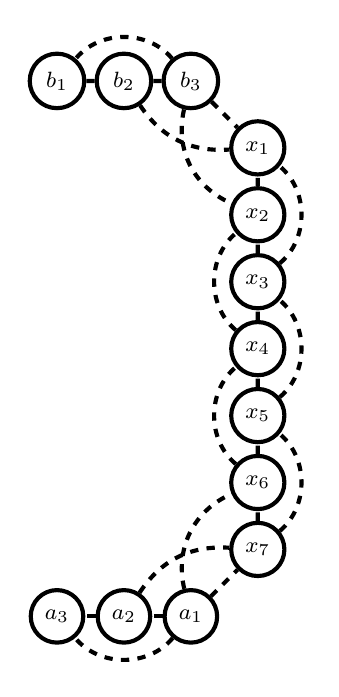
\begin{tikzpicture}[scale=0.85]
    \node[circle, draw=black, fill=white, line width=1.5pt, font=\footnotesize] (a2) at (0, 0) {$a_{3}$};
    \node[circle, draw=black, fill=white, line width=1.5pt, font=\footnotesize] (a1) at (1, 0) {$a_{2}$};
    \node[circle, draw=black, fill=white, line width=1.5pt, font=\footnotesize] (a0) at (2, 0) {$a_{1}$};

    \node[circle, draw=black, fill=white, line width=1.5pt, font=\footnotesize] (b2) at (0, 8) {$b_1$};
    \node[circle, draw=black, fill=white, line width=1.5pt, font=\footnotesize] (b1) at (1, 8) {$b_2$};
    \node[circle, draw=black, fill=white, line width=1.5pt, font=\footnotesize] (b0) at (2, 8) {$b_3$};
    
    \node[circle, draw=black, fill=white, line width=1.5pt, font=\footnotesize] (x1) at (3, 1) {$x_{7}$};
    \node[circle, draw=black, fill=white, line width=1.5pt, font=\footnotesize] (x2) at (3, 2) {$x_{6}$};
    \node[circle, draw=black, fill=white, line width=1.5pt, font=\footnotesize] (x3) at (3, 3) {$x_{5}$};
    \node[circle, draw=black, fill=white, line width=1.5pt, font=\footnotesize] (x4) at (3, 4) {$x_{4}$};
    \node[circle, draw=black, fill=white, line width=1.5pt, font=\footnotesize] (x5) at (3, 5) {$x_{3}$};
    \node[circle, draw=black, fill=white, line width=1.5pt, font=\footnotesize] (x6) at (3, 6) {$x_{2}$};
    \node[circle, draw=black, fill=white, line width=1.5pt, font=\footnotesize] (x7) at (3, 7) {$x_{1}$};
    
    \draw[line width=1.5pt, dashed] (a0) to (a1);
    \draw[line width=1.5pt, dashed] (a1) to (a2);
    \draw[line width=1.5pt, bend left=50, dashed] (a0) to (a2);

    \draw[line width=1.5pt, dashed] (b0) to (b1);
    \draw[line width=1.5pt, dashed] (b1) to (b2);
    \draw[line width=1.5pt, bend right=50, dashed] (b0) to (b2);


    \draw[line width=1.5pt, dashed] (x1) to (x2);
    \draw[line width=1.5pt, dashed] (x2) to (x3);
    \draw[line width=1.5pt, dashed] (x3) to (x4);
    \draw[line width=1.5pt, dashed] (x4) to (x5);
    \draw[line width=1.5pt, dashed] (x5) to (x6);
    \draw[line width=1.5pt, dashed] (x6) to (x7);

    \draw[line width=1.5pt, bend right=50, dashed] (x1) to (x3);
    \draw[line width=1.5pt, bend left=50, dashed] (x2) to (x4);
    \draw[line width=1.5pt, bend right=50, dashed] (x3) to (x5);
    \draw[line width=1.5pt, bend left=50, dashed] (x4) to (x6);
    \draw[line width=1.5pt, bend right=50, dashed] (x5) to (x7);

    \draw[line width=1.5pt, dashed] (a0) to (x1);
    \draw[line width=1.5pt, bend left=40, dashed] (a0) to (x2);
    \draw[line width=1.5pt, dashed, bend left=30,] (a1) to (x1);

    \draw[line width=1.5pt, dashed] (b0) to (x7);
    \draw[line width=1.5pt, bend right=40, dashed] (b0) to (x6);
    \draw[line width=1.5pt, dashed, bend right=30] (b1) to (x7);
\end{tikzpicture}
        \end{figure}
    \end{column}
\end{columns}
\end{frame}


%--------------------------------------------

% \begin{frame}{}
%     We now have \((r-1) \cdot (3k-2)\) vertices.\\
%     Vertices connected paths of length \(n-3\) in configuration graph \\
%     Each connection adds \(4k-2\) vertices\\
%     Configuration graph has now diameter
%     \vspace{-1em}
%     \[(4k-2)(r-1)+\sum d_i\]
%     \begin{columns}
%     \begin{column}{0.6\textwidth}
%         We can use a shortcut to skip \(b_1\) altogether.\\
%         Symmetrically we can do the same on the other side skipping \(a_3\).\\
%         \only<7>{
%         Thus we reduced each connection by 2.\\
%         Finally we obtain:
%             \[(4k-4)(r-1)+\sum d_i\]
%         }
%     \end{column}
%     \begin{column}{0.4\textwidth}
%     \begin{figure}
%         \centering
%         \only<1-2>{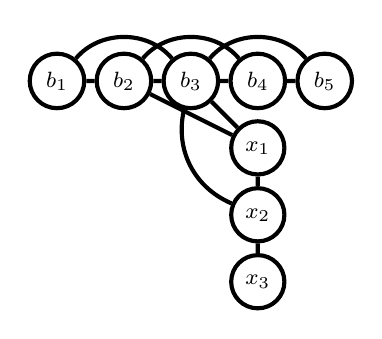
\begin{tikzpicture}[scale=0.85]

    \node[circle, draw=black, fill=white, line width=1.5pt, font=\footnotesize] (b2) at (0, 2) {$b_1$};
    \node[circle, draw=black, fill=white, line width=1.5pt, font=\footnotesize] (b1) at (1, 2) {$b_2$};
    \node[circle, draw=black, fill=white, line width=1.5pt, font=\footnotesize] (b0) at (2, 2) {$b_3$};
    
    \node[circle, draw=black, fill=white, line width=1.5pt, font=\footnotesize] (x5) at (3, -1) {$x_{3}$};
    \node[circle, draw=black, fill=white, line width=1.5pt, font=\footnotesize] (x6) at (3, 0) {$x_{2}$};
    \node[circle, draw=black, fill=white, line width=1.5pt, font=\footnotesize] (x7) at (3, 1) {$x_{1}$};
    

    \draw[line width=1.5pt] (b0) to (b1);
    \draw[line width=1.5pt] (b1) to (b2);
    \draw[line width=1.5pt, bend right=50] (b0) to (b2);


    \draw[line width=1.5pt] (x5) to (x6);
    \draw[line width=1.5pt] (x6) to (x7);

    \draw[line width=1.5pt] (b0) to (x7);
    \draw[line width=1.5pt, bend right=40] (b0) to (x6);
    \draw[line width=1.5pt] (b1) to (x7);
    
    \onslide<2>{
        \node[circle, draw=black, fill=white, line width=1.5pt, font=\footnotesize] (b3) at (3, 2) {$b_4$};
        \node[circle, draw=black, fill=white, line width=1.5pt, font=\footnotesize] (b4) at (4, 2) {$b_5$};
        \draw[line width=1.5pt] (b0) to (b3);
        \draw[line width=1.5pt] (b3) to (b4);
        \draw[line width=1.5pt, bend left=50] (b1) to (b3);
        \draw[line width=1.5pt, bend left=50] (b0) to (b4);
    }
\end{tikzpicture}
}
\only<3>{\begin{tikzpicture}[scale=0.85]

    \node[circle, draw=black, fill=white, line width=1.5pt, font=\footnotesize] (b2) at (0, 2) {$b_1$};
    \node[circle, draw=black, fill=white, line width=1.5pt, font=\footnotesize] (b1) at (1, 2) {$b_2$};
    \node[circle, draw=black, fill=cfred, line width=1.5pt, font=\footnotesize] (b0) at (2, 2) {$b_3$};
    
    \node[circle, draw=black, fill=white, line width=1.5pt, font=\footnotesize] (x5) at (3, -1) {$x_{3}$};
    \node[circle, draw=black, fill=white, line width=1.5pt, font=\footnotesize] (x6) at (3, 0) {$x_{2}$};
    \node[circle, draw=black, fill=white, line width=1.5pt, font=\footnotesize] (x7) at (3, 1) {$x_{1}$};
    

    \draw[line width=1.5pt] (b0) to (b1);
    \draw[line width=1.5pt] (b1) to (b2);
    \draw[line width=1.5pt, bend right=50] (b0) to (b2);


    \draw[line width=1.5pt] (x5) to (x6);
    \draw[line width=1.5pt] (x6) to (x7);

    \draw[line width=1.5pt] (b0) to (x7);
    \draw[line width=1.5pt, bend right=40] (b0) to (x6);
    \draw[line width=1.5pt] (b1) to (x7);
    
        \node[circle, draw=black, fill=cfred, line width=1.5pt, font=\footnotesize] (b3) at (3, 2) {$b_4$};
        \node[circle, draw=black, fill=cfred, line width=1.5pt, font=\footnotesize] (b4) at (4, 2) {$b_5$};
        \draw[line width=1.5pt] (b0) to (b3);
        \draw[line width=1.5pt] (b3) to (b4);
        \draw[line width=1.5pt, bend left=50] (b1) to (b3);
        \draw[line width=1.5pt, bend left=50] (b0) to (b4);
\end{tikzpicture}
}
\only<4>{\begin{tikzpicture}[scale=0.85]

    \node[circle, draw=black, fill=white, line width=1.5pt, font=\footnotesize] (b2) at (0, 2) {$b_1$};
    \node[circle, draw=black, fill=cfred, line width=1.5pt, font=\footnotesize] (b1) at (1, 2) {$b_2$};
    \node[circle, draw=black, fill=cfred, line width=1.5pt, font=\footnotesize] (b0) at (2, 2) {$b_3$};
    
    \node[circle, draw=black, fill=white, line width=1.5pt, font=\footnotesize] (x5) at (3, -1) {$x_{3}$};
    \node[circle, draw=black, fill=white, line width=1.5pt, font=\footnotesize] (x6) at (3, 0) {$x_{2}$};
    \node[circle, draw=black, fill=white, line width=1.5pt, font=\footnotesize] (x7) at (3, 1) {$x_{1}$};
    

    \draw[line width=1.5pt] (b0) to (b1);
    \draw[line width=1.5pt] (b1) to (b2);
    \draw[line width=1.5pt, bend right=50] (b0) to (b2);


    \draw[line width=1.5pt] (x5) to (x6);
    \draw[line width=1.5pt] (x6) to (x7);

    \draw[line width=1.5pt] (b0) to (x7);
    \draw[line width=1.5pt, bend right=40] (b0) to (x6);
    \draw[line width=1.5pt] (b1) to (x7);
    
        \node[circle, draw=black, fill=cfred, line width=1.5pt, font=\footnotesize] (b3) at (3, 2) {$b_4$};
        \node[circle, draw=black, fill=cfred!20, line width=1.5pt, font=\footnotesize] (b4) at (4, 2) {$b_5$};
        \draw[line width=1.5pt] (b0) to (b3);
        \draw[line width=1.5pt] (b3) to (b4);
        \draw[line width=1.5pt, bend left=50] (b1) to (b3);
        \draw[line width=1.5pt, bend left=50] (b0) to (b4);
\end{tikzpicture}
}
\only<5>{\begin{tikzpicture}[scale=0.85]

    \node[circle, draw=black, fill=white, line width=1.5pt, font=\footnotesize] (b2) at (0, 2) {$b_1$};
    \node[circle, draw=black, fill=cfred, line width=1.5pt, font=\footnotesize] (b1) at (1, 2) {$b_2$};
    \node[circle, draw=black, fill=cfred, line width=1.5pt, font=\footnotesize] (b0) at (2, 2) {$b_3$};
    
    \node[circle, draw=black, fill=white, line width=1.5pt, font=\footnotesize] (x5) at (3, -1) {$x_{3}$};
    \node[circle, draw=black, fill=white, line width=1.5pt, font=\footnotesize] (x6) at (3, 0) {$x_{2}$};
    \node[circle, draw=black, fill=cfred, line width=1.5pt, font=\footnotesize] (x7) at (3, 1) {$x_{1}$};
    

    \draw[line width=1.5pt] (b0) to (b1);
    \draw[line width=1.5pt] (b1) to (b2);
    \draw[line width=1.5pt, bend right=50] (b0) to (b2);


    \draw[line width=1.5pt] (x5) to (x6);
    \draw[line width=1.5pt] (x6) to (x7);

    \draw[line width=1.5pt] (b0) to (x7);
    \draw[line width=1.5pt, bend right=40] (b0) to (x6);
    \draw[line width=1.5pt] (b1) to (x7);
    
        \node[circle, draw=black, fill=cfred!20, line width=1.5pt, font=\footnotesize] (b3) at (3, 2) {$b_4$};
        \node[circle, draw=black, fill=white, line width=1.5pt, font=\footnotesize] (b4) at (4, 2) {$b_5$};
        \draw[line width=1.5pt] (b0) to (b3);
        \draw[line width=1.5pt] (b3) to (b4);
        \draw[line width=1.5pt, bend left=50] (b1) to (b3);
        \draw[line width=1.5pt, bend left=50] (b0) to (b4);
\end{tikzpicture}
}
\only<6>{\begin{tikzpicture}[scale=0.85]

    \node[circle, draw=black, fill=white, line width=1.5pt, font=\footnotesize] (b2) at (0, 2) {$b_1$};
    \node[circle, draw=black, fill=cfred!20, line width=1.5pt, font=\footnotesize] (b1) at (1, 2) {$b_2$};
    \node[circle, draw=black, fill=cfred, line width=1.5pt, font=\footnotesize] (b0) at (2, 2) {$b_3$};
    
    \node[circle, draw=black, fill=white, line width=1.5pt, font=\footnotesize] (x5) at (3, -1) {$x_{3}$};
    \node[circle, draw=black, fill=cfred, line width=1.5pt, font=\footnotesize] (x6) at (3, 0) {$x_{2}$};
    \node[circle, draw=black, fill=cfred, line width=1.5pt, font=\footnotesize] (x7) at (3, 1) {$x_{1}$};
    

    \draw[line width=1.5pt] (b0) to (b1);
    \draw[line width=1.5pt] (b1) to (b2);
    \draw[line width=1.5pt, bend right=50] (b0) to (b2);


    \draw[line width=1.5pt] (x5) to (x6);
    \draw[line width=1.5pt] (x6) to (x7);

    \draw[line width=1.5pt] (b0) to (x7);
    \draw[line width=1.5pt, bend right=40] (b0) to (x6);
    \draw[line width=1.5pt] (b1) to (x7);
    
        \node[circle, draw=black, fill=white, line width=1.5pt, font=\footnotesize] (b3) at (3, 2) {$b_4$};
        \node[circle, draw=black, fill=white, line width=1.5pt, font=\footnotesize] (b4) at (4, 2) {$b_5$};
        \draw[line width=1.5pt] (b0) to (b3);
        \draw[line width=1.5pt] (b3) to (b4);
        \draw[line width=1.5pt, bend left=50] (b1) to (b3);
        \draw[line width=1.5pt, bend left=50] (b0) to (b4);
\end{tikzpicture}
}
\only<7>{\begin{tikzpicture}[scale=0.85]

    \node[circle, draw=black, fill=white, line width=1.5pt, font=\footnotesize] (b2) at (0, 2) {$b_1$};
    \node[circle, draw=black, fill=white, line width=1.5pt, font=\footnotesize] (b1) at (1, 2) {$b_2$};
    \node[circle, draw=black, fill=cfred!20, line width=1.5pt, font=\footnotesize] (b0) at (2, 2) {$b_3$};
    
    \node[circle, draw=black, fill=cfred, line width=1.5pt, font=\footnotesize] (x5) at (3, -1) {$x_{3}$};
    \node[circle, draw=black, fill=cfred, line width=1.5pt, font=\footnotesize] (x6) at (3, 0) {$x_{2}$};
    \node[circle, draw=black, fill=cfred, line width=1.5pt, font=\footnotesize] (x7) at (3, 1) {$x_{1}$};
    

    \draw[line width=1.5pt] (b0) to (b1);
    \draw[line width=1.5pt] (b1) to (b2);
    \draw[line width=1.5pt, bend right=50] (b0) to (b2);


    \draw[line width=1.5pt] (x5) to (x6);
    \draw[line width=1.5pt] (x6) to (x7);

    \draw[line width=1.5pt] (b0) to (x7);
    \draw[line width=1.5pt, bend right=40] (b0) to (x6);
    \draw[line width=1.5pt] (b1) to (x7);
    
        \node[circle, draw=black, fill=white, line width=1.5pt, font=\footnotesize] (b3) at (3, 2) {$b_4$};
        \node[circle, draw=black, fill=white, line width=1.5pt, font=\footnotesize] (b4) at (4, 2) {$b_5$};
        \draw[line width=1.5pt] (b0) to (b3);
        \draw[line width=1.5pt] (b3) to (b4);
        \draw[line width=1.5pt, bend left=50] (b1) to (b3);
        \draw[line width=1.5pt, bend left=50] (b0) to (b4);
\end{tikzpicture}
}
%     \end{figure}
%     \end{column}
%     \end{columns}

% \end{frame}

%--------------------------------------------

\begin{frame}{What did we prove?}
    \begin{lemma}{Gluing Lemma}
        Let \(k \geq 3\). Let \(G\) be a graph on \(n\) vertices whose \(k\)-configuration graph contains \(r\) connected components. Then, there exists a graph on at most \(n+(3k-2)\cdot (r-1)\) vertices whose configuration graph had diameter at least \((4k-2)(r-1)+\sum d_i\)
    \end{lemma}

\end{frame}

%--------------------------------------------

\begin{frame}{Recap}
    \begin{theorem}{Upper bound for k=3}
        \[D(n,3)=\Omega(n^2/e^{O(\sqrt{\log n})})\]
    \end{theorem}
    \begin{heading}{Summary of the proof:}
    \begin{itemize}
        \item We construct a graph whose reconfiguration graph is the disjoint union of \(n/e^{o(\sqrt{\log n})}\) paths of linear length by using 3-AP free sets.
        \item We proved that we can add not many vertices to this graph to connect it and make the diameter sum of the components.
    \end{itemize}
    \end{heading}
\end{frame}
% \section{General lower bound}
\section{Conclusions}
\begin{frame}{General bound}
\only<1>{
\begin{theorem}{Theorem}
        \[D(n,k)=\frac{n^{2 \lfloor k /3 \rfloor}}{e^{O_k(\sqrt{\log n})}}\]
\end{theorem}
}
\begin{lemma}{Lemma}
    Let \(n,k\) be two integers. Let \(G\) be a graph with maximum independent sets of size \(k\) such that the \(k\) configuration graph of \(G\) has diameter \(d\). Then, there exists a graph on at most \(|V(G)|+3kn\) vertices whose \(k+3\) reconfiguration diameter is at least \(\frac{dn^2}{e^{O(\sqrt{log n})}}\).
\end{lemma}
\pause
\begin{heading}{Construction idea}
\begin{itemize}
    \item We take graph \(G\) with k-reconfiguration diameter \(d\)
    \item We take graph \(H\) constructed as for \(k=3\).
\end{itemize}
\end{heading}
\end{frame}
% f
\begin{frame}{Just one more proof, I swear}
    \begin{lemma}{Lemma}
        Let \(G\) be a graph. There exists a super-graph \(G'\) of \(G\) with the same number of vertices such that \(R_3(G')\) is a path and the largest diameters of the connected components of \(R_3(G)\) and \(R_3(G')\) are the same.
    \end{lemma}
\end{frame}
\begin{frame}
    \begin{itemize}
        \item \(P\) - diameter path
        \item \(Z=\set{u,v,w}\): node in \(R_3(G)\) not in \(P\)
    \end{itemize}
We show that adding edges outside of the path doesn't change the diameter.
\begin{proof}{Proof}
By contradiction, assume that for any \(x \neq y \in Z\), adding edge \(xy\) to \(G\) decreases the diameter. Thus Each pair from \(Z\) must appear in some independent set within \(P\).

\vspace{0.3cm}

$P$ contains three independent sets:
\begin{itemize}
    \item $\{u, v, a\}$, $\{u, w, b\}$, $\{v, w, c\}$ 
    \item These are neighbours of $Z$ in $\mathcal{R}_3(G)$
    \item By shortest path property: they're consecutive $\Rightarrow a = b = c$
\end{itemize}

But then $\{u,v,a\}$, $\{v,w,a\}$, $\{u,w,a\}$ form a triangle in $\mathcal{R}_3(G)$.

\textbf{Contradiction:} $P$ is an induced path.

\end{proof}

\end{frame}
\begin{frame}{}
    \begin{lemma}{Lemma}
        Let \(G\) be a graph. There exists a super-graph \(G'\) of \(G\) with the same number of vertices such that \(R_3(G')\) is a path and the largest diameters of the connected components of \(R_3(G)\) and \(R_3(G')\) are the same.
    \end{lemma}
    \begin{Lemma}{Conjecture}
        For every \(k \geq 2\) and every \(n\), there exists a graph \(G\) on \(n\) vertices maximising \(D(n,k)\) such that \(R_k(G)\) is a path.
    \end{Lemma}
\end{frame}
\begin{frame}{Open problems}
    \begin{fact}{Conjecture} 
        \(D(n,4)=n^{3-o(1)}\) - we can find \(R_4(G)\) with super-quadratic diameter.
    \end{fact}
    \pause
    \begin{fact}{Conjecture}
        For every \(k \geq 2\) and every \(n\), there exists a graph \(G\) on \(n\) vertices maximising \(D(n,k)\) such that \(R_k(G)\) is a path.
    \end{fact}
    \pause
    \begin{fact}{Question}
        What is the asymptotic behaviour of \(\max_k D(n,k)\)?
    \end{fact}
    \pause
    \begin{fact}{Question}
        Is finding largest possible diameter of \(R_3(G)\) equivalent to \((6,3)\) problem?
    \end{fact}
    \vspace{1em}
    \pause
    \begin{figure}
        \centering
        \Large\textcolor{cfred}{Thanks!}
    \end{figure}
\end{frame}
%---------------------------------------------------------
% \begin{frame}{Sources}
% \label{references}
%     \begin{itemize}
%         \item Nicolas Bousquet, Bastien Durain, Théo Pierron, Stéphan Thomassé\href{https://arxiv.org/pdf/2301.02020}{\textit{Extremal Independent Set Reconfiguration}}, 2023. \\
%     \end{itemize}

% \end{frame}

%---------------------------------------------------------


\end{document}